\documentclass[a4paper,10pt,ngerman]{scrartcl}
\usepackage{babel}
\usepackage[T1]{fontenc}
\usepackage[utf8x]{inputenc}
\usepackage[a4paper,margin=2.5cm,footskip=0.5cm]{geometry}

% Die nächsten drei Felder bitte anpassen:
\newcommand{\Aufgabe}{Aufgabe 3 - HexMax} % Aufgabennummer und Aufgabennamen angeben
\newcommand{\TeilnahmeId}{60302}                  % Teilnahme-ID angeben
\newcommand{\Name}{Florian Bange}             % Name des Bearbeiter / der Bearbeiterin dieser Aufgabe angeben


% Kopf- und Fußzeilen
\usepackage{scrlayer-scrpage, lastpage}
\setkomafont{pageheadfoot}{\large\textrm}
\lohead{\Aufgabe}
\rohead{Teilnahme-ID: \TeilnahmeId}
\cfoot*{\thepage{}/\pageref{LastPage}}

% Position des Titels
\usepackage{titling}
\setlength{\droptitle}{-1.0cm}

% Für mathematische Befehle und Symbole
\usepackage{amsmath}
\usepackage{amssymb}

% Für Bilder
\usepackage{graphicx}
\graphicspath{ {./images/} }

% Pseudocode
\usepackage{algpseudocode,algorithm,algorithmicx}

% Trees
\usepackage{qtree}

% Für Quelltext
\usepackage{listings}
\usepackage{color}
\definecolor{mygreen}{rgb}{0,0.6,0}
\definecolor{mygray}{rgb}{0.5,0.5,0.5}
\definecolor{mymauve}{rgb}{0.58,0,0.82}
\lstset{
  keywordstyle=\color{blue},commentstyle=\color{mygreen},
  stringstyle=\color{mymauve},rulecolor=\color{black},
  basicstyle=\footnotesize\ttfamily,numberstyle=\tiny\color{mygray},
  captionpos=b, % sets the caption-position to bottom
  keepspaces=true, % keeps spaces in text
  numbers=left, numbersep=5pt, showspaces=false,showstringspaces=true,
  showtabs=false, stepnumber=2, tabsize=2, title=\lstname
}

% Diese beiden Pakete müssen zuletzt geladen werden
%\usepackage{hyperref} % Anklickbare Links im Dokument
\usepackage{cleveref}

% Daten für die Titelseite
\title{\textbf{\Huge\Aufgabe}}
\author{\LARGE Teilnahme-ID: \LARGE \TeilnahmeId \\\\
	    \LARGE Bearbeitet von \\ 
	    \LARGE \Name\\\\}
\date{\LARGE\today}

\begin{document}

\maketitle
\tableofcontents

\vspace{0.5cm}

\section{Einleitung}
Dieses Problem moechte ich loesen, indem ich das gleiche, allgemeinere Problem fuer beliebige Basen (im Folgenden "`a"' genannt) angehe. Das Programm ist fuer die Basis 16 geschrieben.
\\\\
Im Folgenden werden die sieben Positionen einer Siebensegmentanzeige Segmente genannt. Weiter sind "`aktivierte Segmente"' Segmente, welche durch ein "`Staebchen"' belegt sind und "`deaktivierte Segmente"' Segmente, welche frei sind.

\section{Ziffern veraendern}
Um dieses Problem zu loesen, muss man offensichtlich die Ziffern der gegebenen Zahl systematisch veraendern.\\\\
Moechte man eine Siebensegmentanzeige d zu einer anderen Siebensegmentanzeige g veraendern, muss man dafuer Segmente in d aktivieren und/oder deaktivieren.\\
Aktivieren muss man die Segmente, welche in d nicht aktiviert, aber in g aktiviert sind und deaktivieren muss man die Segmente, welche in d aktiviert sind, aber in g nicht.
\\ \\
Der Prozess des Veraenderns einer Ausgangssiebensegmentanzeige d zu einer Zielsiebensegmentanzeige g wird im Folgenden schlicht Veraenderung genannt.
\\
Die Anzahl der Segmente, die aktiviert werden muessen, nenne ich im Folgenden a und die Anzahl der Segmente, die deaktivieren werden muessen r.
\\\\
\textbf{Beispiele}
\begin{enumerate}
	\item
	Moechte man A zu B veraendern - \\ \\
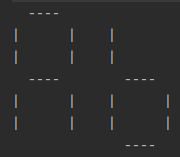
\includegraphics{AB} \\
- muss man zwei Segmente, oben rechts deaktivieren und ein Segment unten aktivieren. Somit ist r=2 und a=1.
	\item
	Moechte man A zu F veraendern - \\ \\
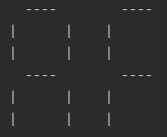
\includegraphics{AF} \\
- muss man zwei Segmente, rechts deaktivieren und keine Segmente aktivieren. Somit ist r=2 und a=0.
	\item
Moechte man 2 zu 5 veraendern - \\ \\
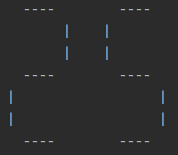
\includegraphics{25} \\
- muss man oben links und unten rechts ein Segment aktivieren und oben rechts und unten links ein Segment deaktivieren. Somit ist r=2 und a=2.
\end{enumerate}
\\\\
Selbstverstaendlich exestiert ebenfalls der Fall, dass r und a gleich 0 sind, falls d = g gilt.
\\
\\
\\
Sei nun
\[changes: (d, \ g) \rightarrow (a, \ r)\]
eine Funktion, welche von Tupeln an Ziffern (d und g) abbildet auf Tupel der natuerlichen Zahlen mit null (a, r).\\\\
Dabei stellt d die Ziffer der Ausgangssiebensegmentanzeige und g die Ziffer der Zielsiebensegmentanzeige dar. a ist die Anzahl der Segmente, welche aktiviert werden muessen und r die Anzahl der Segmente, welche deaktiviert werden muessen, 
um von d's Siebensegmentanzeige zu g's Siebensegmentanzeige zu kommen.\\\\
\textbf{Pseudocode}\\
Der Pseudocode zum erhalten von den Werten \(a\) und \(r\) fuer zwei Ziffern \(d\) und \(g\) sieht wie folgt aus:
\begin{algorithmic}[1]
\Procedure {getAddAndRemove}{\(d, \ g\)}
		\State \(segmentD_1, \ \dots \ , \ segmentD_7\) \gets \(getSegments(d)\)
		\State \(segmentG_1, \ \dots \ , \ segmentG_7\) \gets \(getSegments(g)\)
		\State \(a\) \gets \(0\)
		\State \(r\) \gets \(0\)
		\State 
		\For{\(i \gets 1 \ \textbf{to} \ 7\)} \Comment{Go through segments}
					\If {\(segmentD_i \ \textbf{and} \ \textbf{not} \ segmentG_i\)}
							\State \(r\) \gets \(r+1\)
					\Else {\( \ \textbf{not} \ segmentD_i \ \textbf{and} \  segmentG_i\)}
							\State \(a\) \gets \(a+1\)
					\EndIf
		\EndFor
		\State
		\State \textbf{return} \((a, \ r)\)
\EndProcedure
\end{algorithmic}
\\\\
Die Methode \(getSegments\) soll hier eine Methode darstellen, welche die sieben Segmente der Siebensegmentanzeige einer Ziffer als Wahrheitswert zurueckgibt.\\\\
Die soeben beschriebene Vorgehensweise kann ebenfalls benutzt werden, um herrauszufinden, welche Segmente (bestimmt durch ihren Index) aktiviert/deaktiviert werden muessen, um von \(d\) zu \(g\) zu kommen.

\section{Reihenfolge der Veraenderungen}
Es ist leicht erkennbar, dass man versuchen sollte, die Ziffern von links nach rechts zu erhoehen. Denn fuer eine Zahl mit den Ziffern \(d_n, \ d_{n-1}, \ \dots \ , \ d_2, \ d_1\) (von links nach rechts in dieser Reihenfolge - absteigend nummeriert) hat eine Ziffer an Index \(i\) (\(1 \leq i \leq n\)) schon bei Erhoehung um eins mehr Einfluss auf den Wert der Zahl, als wuerde man alle anderen Ziffern von Index \(1\) bis \(i-1\) auf den hoechsten Wert - \((a-1)\) - setzen.
\\\\
Dies laesst sich wie folgt durch vollstaendige Induktion beweisen.
\\\\
Sein
\[d_n, \ d_{n-1}, \ \dots \ , \ d_2, \ d_1\]
die Ziffern einer Zahl \(m\) mit Basis \(a\), welche \(n\) Ziffern hat. Dabei liegt die Ziffer \(d_n\) ganz links in der Zahl und die Ziffer \(d_1\) ganz rechts in der Zahl. Die Ziffern sind also von rechts nach links aufsteigend nummeriert.
\\\\
Den Wert der Zahl \(m\) kann man als Summe mit Hilfe der Ziffern und der Basis wie folgt darstellen:\\
\[m = \sum_{i=1}^n d_i * a^{i-1}\]
Dabei hat jede Ziffer an Index \(i\) (\(1 \leq i \leq n\)) den Stellenwert \(a^{i-1}\).
\\\\
Sei \(i\) eine natuerliche Zahl mit \(1 \leq i \leq n\).
Nun wird gezeigt, dass der Wert der Stelle \(i\) mit der Ziffer \(1\) groeszer ist als die Summe aller Stellen mit einem Index kleiner als \(i\) mit je der groeszten Ziffer, \(a-1\).\\
Formal (Induktionsvoraussetzung):
\[1 * a^{i-1} > \sum_{k=1}^{i-1} (a-1) * a^{k-1}\]
Induktions Anfang (\(i = 1\))
\[1 * a^{1-1} = a^{1-1} = a^0 = 1 > 0 = \sum_{k=1}^0 (a-1)*a^{k-1} = \sum_{k=1}^{1-1} (a-1)*a^{k-1}\]
Induktionsbehauptung:
\[1 * a^{(i+1)-1} > \sum_{k=1}^{(i+1)-1} (a-1) * a^{k-1}\]
Induktionsschritt:
\[1 * a^{(i+1)-1} = a^{i} = a * a^{i-1} = (a-1) * a^{i-1} + a^{i-1} \overset{IV}{>} (a-1) * a^{i-1} + \sum_{k=1}^{i-1} (a-1) * a^{k-1} = \sum_{k=1}^{i} (a-1) * a^{k-1} = \sum_{k=1}^{(i+1)-1} (a-1) * a^{k-1}\]

\section{Eigenschaften einer korrekten Loesung}
Damit eine Zahl eine korrekte Loesung ist, muss Folgendes gegeben sein:
\begin{enumerate}
	\item Die Zahl ist gueltig (jede Ziffer existiert in der Basis)
	\item Die Anzahl der Segmente ist die gleiche wie bei der gegebenen Zahl
	\item Die gegebene Maximalzahl an Umlegungen ist nicht ueberschritten
	\item Die Zahl ist groeszer als die gegebene Zahl oder gleich grosz
\end{enumerate}

\section{Schluesse aus der korrekten Loesung}
Sein \(d_n, \ \dots \ , \ d_1\) die Ziffern der gegeben Zahl von links nach rechts und \(d_n', \ \dots \ , \ d_1'\) die jeweiligen Ziffern der korrekten Loesung. Weiter sind \(a_i\) und \(r_i\) die Anzahl an Segmenten, 
die man hinzufuegen, bzw. entfernen muss um von \(d_is\) Siebensegmentanzeige zu \(d_i's\) Siebensegmentanzeige zu kommen (\(1 \leq i \leq n\)), bzw.
\[(a_i, \ r_i) = changes(d_i, \ d_i')\]
fuer alle \(i \in \mathbb{N}\) mit (\(1 \leq i \leq n\)).
\\\\
Weiter sei 
\[A = \sum_{i=1}^n a_i\]
und
\[R = \sum_{i=1}^n r_i\]
Daraus, dass eine korrekte Loesung, nach den zuvor beschriebenen Punkten gegeben ist, laesst sich Folgendes schlieszen:
\begin{enumerate}

	\item
	\[\sum_{i=1}^n a_i - r_i = 0\]
Dies liegt schlicht daran, dass somit nicht mehr Segmente entfernt oder hinzugefuegt werden muessen als existieren, so dass am Ende gleich viele Segmente vorhanden sind, wie bei der gegebenen Zahl.

	\item A = R\\
	Dies laesst sich aus dem ersten Punkt wie folgt schlieszen:
	\[\sum_{i=1}^n a_i - r_i = 0\]
	\[\Leftrightarrow (a_1 - r_1) + \cdots + (a_n - r_n) = 0\]
	\[\Leftrightarrow a_1 + (-r_1) + \cdots + a_n + (-r_n) = 0\]
	\[\Leftrightarrow a_1 + \cdots + a_n + (-r_1) + \cdots + (-r_n) = 0\]
	\[\Leftrightarrow a_1 + \cdots + a_n - r_1 - \cdots - r_n = 0\]
	\[\Leftrightarrow a_1 + \cdots + a_n - (r_1 + \cdots + r_n) = 0\]
	\[\Leftrightarrow \sum_{i=1}^n a_i - \sum_{i=1}^n r_i = 0\]
	\[\Leftrightarrow A - R = 0\]
	\[\Leftrightarrow A = R\]
	
	\item Man kann benoetigt \(\dfrac{A+R}{2}\) Umlegungen\\
	Dies wird ersicht, da A die Anzahl aller Segmente ist, die hinzugef�gt werden muessen (dort ist also noch kein aktiviertes Segment) und R die Anzahl der Segmente ist, die entfernt werden muessen (dort ist also ein aktiviertes Segment) (um von \(d_1, \ \dots \ , \ d_n\) zu \(d_1', \ \dots \ , \ d_n'\) zu kommen). Nun kann man fuer jedes der R Segmente, die deaktiviert werden muessen, je eines der A Segmente, die aktiviert werden muessen, aktivieren. Dies ist moeglich, da \(A = R\) gelten muss. Somit ergeben sich \(\dfrac{A+R}{2}\) Umlegungen. Bzw., da A gleich R gilt, A = R Umlegungen.
\end{enumerate}
\\\\\\\\

\section{Modellierung}
Sei eine Zahl der Basis a mit n Ziffern gegeben. Die Ziffern seien nun \(d_1, \ \dots \ , \ d_n\) (\(d_1\) ganz links, \(d_n\) ganz rechts).\\\\
Alle moeglichen Belegungen der Ziffern \(d_1, \ \dots \ , \ d_n\) lassen sich als Baum darstellen.\\\\
Dabei ist die Wurzel auf Level 0 des Baums leer.\\
Fuer jeden Index \(i\) der Zahl (\(1 \leq i \leq n\)) gehen auf Level \(i - 1\) stets a Pfade von jedem Knoten auf Level \(i-1\) zu je einem Knoten auf Level \(i\) ab. Diese \(a\) Knoten Stellen je alle \(a\) Ziffern der Basis \(a\) (\(0, \ \dots \ , \ a-1\)) dar.\\\\
Jeder Knoten auf Level i enthaelt eine Ziffer g, sowie das Tupel \(changes(d_i, \ g)\)\\\\
Die Anzahl an Blaettern ist demnach \(a^n\) und die Hoehe ist \(n+1\). \\\\
Ein Beispiel Baum zur Zahl 12 der Basis 3 (n ist somit 2) ist:
\begin{center}
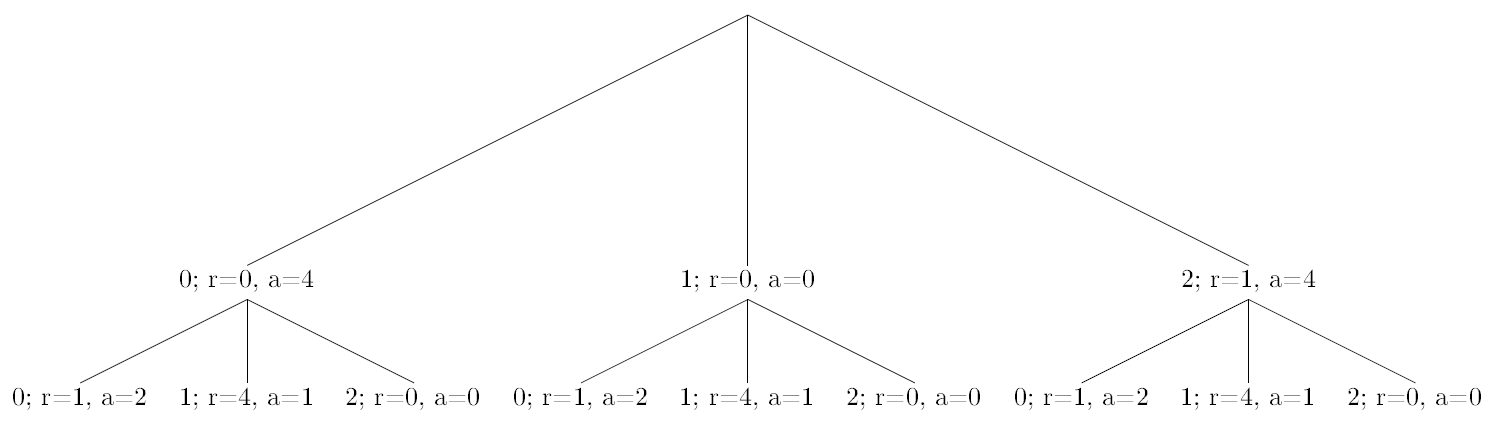
\includegraphics[width=15cm]{12_B3-Graph}
\end{center}
In einem solchen Baum waere nun die Aufgabe, den Pfad zu finden, bei dem die Summe A aller a's der Summe R aller r's entspricht.\\
Und fuer diese Summen gilt, dass sie beide nicht groeszer sind als die Maximalanzahl an Veraenderungen.\\\\
Selbstverstaendlich soll dabei der Pfad gefunden werden, der als Zahl den groeszten Wert hat. Dazu koennte man die a Knoten, welche die a Ziffern der Basis a darstellen, immer absteigend (wie im Beispiel) oder immer aufsteigend hinzufuegen. Dann muesste man nur von rechts nach links bzw. von links nach rechts eine Tiefensuche durchfuehren und den ersten Pfad waehlen, welcher die zuvor beschriebene Eigenschaften hat.

\section{Rekursiver Algorithmus}
Im Folgenden Loesungsweg wird ausschlieszlich die Berechnung der hoechsten Zahl umgesetzt ohne die Umlegungen zu beachten. Denn diese koennen deutlich einfacher im Nachhinein berechnet werden. Dazu spaeter mehr.\\\\
Aus der Darstellung als Baum kann man vermuten, dass sich das HexMax-Problem rekursiv formulieren laesst. Tatsaechlich ist dies wie folgt moeglich:\\\\
Geben ist erneut die Zahl der Basis a mit den n Ziffern \(d_1, \ \dots \ , \ d_n\) und die Maximalzahl an Veraenderungen m.
\\\\
Fuer den rekusiven Algorithmus sein nun folgende Eingabeparamether gegeben:
\begin{enumerate}
	\item Ein momentaner Index einer Ziffer: index (\(1 \leq index \leq n\))
	\item Die momentane Gesamtanzahl an Segmenten, die hinzugefuegt werden muessen: A
	\item Die momentane Gesamtanzahl an Segmenten, die entfernt werden muessen: R
\end{enumerate}
Der Rueckgabewert soll eine Liste an Ziffern der Groesze \(n - index + 1\) oder NULL sein. NULL stellt den Fall dar, dass keine Loesung gefunden wird.
\\\\
Die Aufgabe des Algorithmus lautet, ab dem gegebenen Index (inklusive index) die hoechste Belegung der Ziffern zu finden, welche die benoetigten Eigenschaften erfuehlt: \(A = R \leq m\)
\\\\
Rekursion kann hier sehr schoen angewendet werden, indem an jedem Aufruf an einem Index i, alle moeglichen Ziffern g der Basis a absteigend durchgegangen werden. Dazu wird dann \((a, \ r) = changes(d_i, \ g)\) berechnet und die Funktion rekursiv benutzt, wobei als naechster Index index+1, als naechstes A A+a und als naechstes R R+r genommen werden.\\
Sollte der Rueckgabewert des rekursiven Aufrufs NULL sein, so wird die naechstkleinere moegliche Ziffer probiert. Sollte der Rueckgabewert nicht NULL sein, wird eine Liste erzeugt, welche an erster Position g hat und weiter mit dem Rueckgabewert gefuellt ist. Diese wird zurueckgegeben.\\\\
Sollte, nachdem alle Ziffern der Basis a absteigend durchgegangen wurden, jeder rekursive Aufruf NULL ergeben haben, so wird NULL zurueckgegeben.
\\\\
Die Abbruchbedingungen des rekursiven Algorithmus stellen dar:
\begin{enumerate}
	\item A+R ist groeszer als 2 * m\\
	In diesem Fall wuerden zu viele Umlegungen gebraucht, so dass NULL zurueckgegeben werden muss.\\
	Denn, wie aus korrekten Loesungen geschlossen wurde, muss \(A = R \leq m\) gelten. Dies laesst sich zu \(2A = 2R \leq 2m\) umformen. Dies wiederum entspricht \(A + R \leq 2m\), da \(A = R\) sein muss.
	
	\item Ein zu groszer Index, bzw. ein Index der groeszer als n ist\\
	In diesem Fall wird ueberprueft, ob \(A = R\) und \(A \leq m\) bzw. \(R \leq m\) gilt, nur dann wird eine leere Liste zurueckgegeben, sonst wird NULL zurueckgegeben.\\
	Wird die Reihenfolge, wie hier nummeriert benutzt, kann die Abfrage nach \(A \leq m\) bzw. \(R \leq m\)
	natuerlich weggelassen werden, da sie durch Punkt 1 gegeben ist.
	
	\item \(A+R\) ist genau gleich \(2*m\)\\ 
	Ist dies der Fall, so ist die Anzahl an Umlegungen genau erreicht. Weiter muss zusaetzlich ueberprueft werden, ob \(A=R\) gilt.\\
	Ist dies gegeben, wird eine Teilmenge der Ziffern ab Index index (inklusive index) zurueckgegeben.
\end{enumerate}

\section{Loesung durch Dynamische Programmierung}
Der soeben beschriebene Algorithmus loest zwar das Problem, indem die Uebergabeparamether \(index = 1, A = 0\) und \(R = 0\) benutzt werden, hat aber eine deutlich zu hohe Laufzeit von maximal ca. \(a^n\).\\
Dies ergibt sich daraus, dass so maximal lange gesucht wuerde, bis das Ergebnis gleich der Eingabezahl ist. \\\\
Um diese Laufzeit stark zu senken, kann man einen Blick auf die Anzahl an moeglichen Eingaben fuer die jeweiligen Eingabeparamether werfen:\\\\
\begin{tabular}{ c | c | c}
  index & A & R\\
	\hline
  n & 5n & 5n 
\end{tabular}\\\\\\
Dabei ergeben sich die Werte fuer A und R durch die Maximalzahl an Segmenten, die deaktiviert bzw. aktiviert werden koennen, um eine neue Ziffer zu erstellen: 5. Dies ist bei 1 und 8 der Fall. Multipliziert man diese Maximalzahl der Segmente, die aktiviert/deaktiviert werden koennen mit der Anzahl an Ziffern (n), ergibt sich 5n.\\\\
Multipliziert man die Anzahl an moeglichen Eingaben fuer jeden Eingabeparamether, ergibt sich
\[n * 5n * 5n = 25n^3.\]
Dieser Wert stellt die Maximalzahl an Eingaben fuer den Algorithmus dar.
\\\\
Da dieser Wert deutlich langsamer waechst als \(a^n\), kann man hier Memoisation bzw. Dynamische Programmierung benutzen. Dies bedeutet, dass man bereits berechnete Rueckgabwerte speichert, um sie ggf. wieder benutzen zu koennen.\\
Dazu wird am Anfang des Algorithmus ueberprueft, ob dieselbe Eingabe (index, A und R) bereits gespeichert wurde. Ist dies der Fall, wird das gespeicherte Ergebnis zurueckgegeben.\\
Damit dies moeglich ist, wird der Wert, welcher zurueckgegeben werden wird, gespeichert. Dies ist stets entweder ein Liste oder NULL.
\\\\
\textbf{Pseudocode}\\
Nun folgt der Pseudocode fuer den zuvor beschriebenen rekursiven Algorithmus zusammen mit der Dynamischen Programmierung.\\\\
Gegeben, als feste Werte fuer den Algorithmus sind die Ziffern der Zahl (nun von links nach rechts): \(d_1, \ \dots \ , \ d_n\) ganz links in der Zahl ist \(d_1\) und \(d_n\) ist ganz rechts. Somit hat die Zahl \(n\) Ziffern - dieser Wert ist ebenfalls gegeben.\\
Weiter ist die Maximalanzahl an Umlegungen \(m\) gegeben.\\
Die Eingabeparamether des Algorithmus sind wie beschrieben (index, A, R).\\

% \begin{center}
% \begin{algorithm}
% \caption{Rekursiver algorithmus mit DP}
\begin{algorithmic}[1]
\State memo \gets \([ \ ]\) \Comment{Memoisation object - dictionary}
\Procedure {getHighestNumber}{index, A, R}
	\If{memo.contains(index, A, R)} \Comment{Check if memo contains inputs meaning they were already calculated} 
			\State \textbf{return} memo.get(index, A, R) \Comment{Return them if so} 
	\EndIf	
	\State
	\If{A + R > 2*m} \Comment{Max amount of changes is overstepped, so returning null}
			\State \textbf{return} NULL
	\EndIf		
	\State
	\If{index > n} \Comment{Index of digit is bigger than amount of digits (n)}
			\If{A = R} \Comment{Check \(A = R\), note that \(A+R \leq 2*m\) is given by previous check}
					\State \textbf{return} [ \ ] \Comment{Empty array} 		
			\Else
					\State \textbf{return} NULL
			\EndIf
	\EndIf		
	\State
	\If{A + R = 2*m} \Comment{Max amount of changes exactly reached}
			\If{A = R} \Comment{Check \(A = R\)}
					\State \textbf{return} [\(d_{index}, \ \dots \ , \ d_n\)]
			\Else
					\State \textbf{return} NULL
			\EndIf
	\EndIf		
	\State
	\For{g \gets (a-1) \ \textbf{to} \ 0} \Comment{Go through digits of base a, decreasing}
			\State (adds, removes) \gets changes(\(d_{index}\), \ g)
			\State subResult \gets getHighestNumber(index \(+1\), \ A \(+\) adds, \ R \(+\) removes)
			\If{subResult \(\not=\) NULL}
					\State finalResult \gets \([ \ g \ ]\)
					\State \textbf{add all} subResult \textbf{to} finalResult
					\State memo.put(index, A, R, finalResult) \Comment{Put found result into memo for current inputs}
					\State \textbf{return} finalResult
			\EndIf	
	\EndFor
	\State
	\State memo.put(index, A, R, NULL) \Comment{Put NULL into memo for current inputs}
	\State \textbf{return} NULL
\EndProcedure
\end{algorithmic}
% \end{algorithm}
\\\\\\Wichtig ist zu beachten, dass die Reihenfolge der Abbruchbedingung der Rekursion so gehalten werden, dass stets sicher ist, dass \(A = R \leq m\) gilt.
\\\\Weiter ist das Memoisation Objekt "`memo"' zum speichern der Ergebnisse hier vereinfacht dargestellt. Es sollen index, A und R als Schluessel (keys) und die Liste oder NULL als dazu assozierter Wert (value) gesehen werden. Dazu unter Implementierung genaueres.
\\\\Weiter sei wiederholt, dass dieser Algorithmus mit den Uebergabeparamethern Index = 1, A = 0 und R = 0 das eigentliche Problem loest.

\section{Berechnung der Umlegungen}
Nach dem die hoechstmoegliche Zahl berechnet wurde, kann man mit dieser und der Ausgangszahl die benoetigten Umlegungen berechnen. Dabei muss beachtet werden, dass stets ein aktiviertes Segment mit einem deaktivierten Segment getauscht und niemals eine Siebensegmentanzeige vollstaendig geleert wird. 
\\\\
Gegeben sein die Ziffern der gegebenen Zahl \(d_1, \ \dots \ , \ d_n\) und die Ziffern der resultierenden Zahl \(d_1', \ \dots \ , \ d_n'\).
\\\\
Zunaechst wird fuer jedes Paar (\(d_i\) und \(d_i'\)) die Liste der Segmente, die entfernt werden muessen - \(removes_i\) - und die Liste der Segmente, die hinzugefuegt werden muessen - \(adds_i\), berechnet.\\
Segmente werden dabei ueber ihren Index j (\(0 \leq j < 7\)) definiert.
\\\\
Anschlieszend werden alle Indexe i der Hex-Zahl (\(1 \leq i \leq n\)) durchgegangen. Fuer jeden Index i werden so lange Elemente aus \(adds_i\) mit Elementen aus \(removes_i\) getauscht, wobei bei jedem Tausch die jeweiligen Segmente aus beiden Listen entfernt werden, bis eine Liste leer ist.
\\\\
Als naechstes werden alle restlichen Segmente aus add- und remove-Listen miteinander getauscht, bis alle Listen leer sind.
\\\\
Bei jedem der erwaehnten Taeusche wird dieser gespeichert.\\
Jeder Tausch von zwei Segmenten besteht dabei aus den Indexen der zwei Ziffern und aus den jeweiligen Indexen der Segmente in den Segmenten. Es ist moeglich, dass die Indexe der Ziffern dabei identisch sind.
\\\\
\textbf{Pseudocode}\\
Nun wird der Pseudocode fuer den zuvor beschriebenen Algorithmus folgen.\\
Die Uebergabeparamether sind \(d_1, \ \dots \ , \ d_n\) - die Ziffern der gegebenen Zahl - und \(d_1', \ \dots \ , \ d_n'\) - die Ziffern der resultierenden Zahl.
\begin{algorithmic}[1]
	\Procedure {getNeededChanges}{\(d_1, \ \dots \ , \ d_n\), \(d_1', \ \dots \ , \ d_n'\)}
	\State \(adds_1, \ \dots \ , \ add_n \) \Comment{Declare adds-lists}
	\State \(removes_i, \ \dots \ , \ removes_i \) \Comment{Declare removes-lists}
	\For{i \gets 1 \ \textbf{to} \ n} \Comment{Get remove- and add-stacks for each index i}
			\State \(add_i\) \gets \(neededAdds(d_i, \ d_i')\)
			\State \(removes_i\) \gets \(neededRemoves(d_i, \ d_i')\)
	\EndFor
	\State
	\For{i \gets 1 \ \textbf{to} \ n} \Comment{1. Swap inside of digits}
			\While{\(adds_i.size\) > 0 \textbf{and} \(removes_i.size\) > 0} \Comment{Repeat until one stack is empty}
					\State addSwap(\(add_i.pop(), \ removes_i.pop(), \ i\))
			\EndWhile
	\EndFor
	\State
	\State addIndex \gets \(0\)
	\State removeIndex \gets \(0\)
	\State addStack \gets \([ \ ]\)
	\State removeStack \gets \([ \ ]\)
	\State isDone \gets \(false\)
	\State
	\While {!isDone} \Comment{2. Swap left segments}
			\While {addStack.size > 0 \textbf{and} addIndex \leq n } \Comment{Get next non-empty add stack if current is empty and it's possible}
					\State addIndex \gets \(addIndex + 1\)
					\State addStack \gets \(adds_{addIndex}\)
			\EndWhile
			\State
			\While {\(removeStack.size > 0 \ \textbf{and} \ removeIndex \leq n \)} \Comment{Get next non-empty remove stack if current is empty and it's possible}
					\State removeIndex \gets \(removeIndex + 1\)
					\State removeStack \gets \(removes_{removeIndex}\)
			\EndWhile
			\State
			\If {\(addStack.size = 0\)} \Comment{No swaps are left} 
					\State isDone \gets \(true\)
			\Else
					\State addSwap(\(addIndex, \ add_i.pop(), \ removeIndex, \ removes_i.pop()\))
			\EndIf
	\EndWhile
\State
\EndProcedure
\end{algorithmic}
\\\\
Die removes und adds Listen werden hier ueber die Methoden neededAdds und neededRemoves erhalten. Diese sollen Methoden dastellen, welche fuer zwei Ziffern ausgeben, welche Segmente (bestimmt durch ihren Index) entfernt bzw. hinzugefuegt werden muessen, um von der einen Ziffer zur anderen zu kommen.\\\\
Die removes und adds Listen sollen hier des weiteren Stacks sein, so dass das oberste Element des Stacks mit der pop-Methode bekommen und vom Stack entfernt werden kann.\\
Des weiteren sollen die addSwap Methoden die Taeusche (swaps) speichern. \\
Zu beidem unter Implementierung genaueres.
\\\\
Warum dieses Verfahren korrekt ist, wird unter Korrektheit argumentiert.

\section{Optimierung}
Optimieren kann man diesen Loesungsweg durch Folgendes:
\begin{enumerate}
	\item Es sollten alle Ergebnisse der changes-Funktion bereits vorgeneriet sein, so dass r und a nicht jedes Mal neu berechnet werden muessen.
	Genauer sollte fuer jedes Paar an Ziffern der Basis a die Liste an Segmenten (bzw. deren Indexe), welche hinzugefuegt/entfernt werden, vorgeneriert werden, so dass diese im Laufe des Programs nicht mehrmals berechnet werden.
\end{enumerate}

\section{Korrektheit}
Die Korrektheit werde ich nun Punkt fuer Punkt begruenden.
\\\\
\textbf{Zunaechst zur Korrektheit der Berechnung der Umlegungen.}\\
Hier ist zu beachten, dass eine Siebensegmentanzeige niemals vollkommen leer sein darf. Es muss also jede immer mindestens ein aktiviertes Segment enthalten.
\\\\
Im ersten Teil der Berechnung wird niemals eine Anzeige leer sein, da die Anzahl an aktivierten Segmenten in einer Anzeige die gleiche bleibt, wenn man eine Umlegung innerhalb der Anzeige vornimmt.
\\
Im zweiten Teil der Berechnung gibt es fuer jede Ziffer an Index i drei Moeglichkeiten:
\begin{enumerate}
	\item Es wird nichts nach auszen veraendert, da die Ziffer \(d_i'\) bereits erreicht ist.\\
	In diesem Fall kann die Anzeige nicht leer werden, da nichts veraendert wird.
	\item \(a_i < r_i\) - Es muessen \(-(a_i \ - \ r_i)\) Segmente entfernt werden, so dass diese zu anderen Ziffern hinzugefuegt werden.\\
	In diesem Fall wird es niemals dazu kommen, dass die Anzeige an Index i vollkommen leer wird. Denn es ist sicher, dass durch das Entfernen der Segmente eine neue Ziffer entsteht. Und jede Ziffer besitzt aktivierte Segmente.
	\item \(a_i > r_i\) - Es muessen \(a_i - r_i\) Segmente hinzugefuegt werden, sodass diese von anderen genommen werden muessen.\\
	In diesem Fall werden Segmente hinzugefuegt, sodass die Anzahl der aktivierten Segmente nicht kleiner wird und die Anzeige niemals leer wird.
\end{enumerate}
\\\\
\textbf{Nun zur Korrektheit des rekursiven Algorithmus mit der Dynamischen Programmierung.}
\begin{enumerate}
	\item Die Anzahl an Umlegungen ist nicht groeszer als vorgegeben durch m.\\
	Dies wird durch die Abbruchbedingung \(A+R > 2*m\) gegeben, welche dafuer sorgt, dass niemals mehr Veraenderungen gebraucht werden als durch Umlegungen moeglich sind.
	
	\item Die Anzahl der Ziffern ist nicht veraendert.\\
	Dies ist gegeben, da in dem Loesungsweg keine Moeglichkeit existiert, Ziffern hinzuzufuegen oder zu entfernen.
	
	\item Die Anzahl der aktivierten Segmente ist die gleiche, wie bei der gegebenen Zahl.\\
	Dies ist gegeben, da in den Abbruchbedingungen stets geprueft wird, dass \(A = R\) ist, sodass gleich viele Segmente aktiviert und deaktiviert werden.

	\item Die Loesung ist groeszer oder gleich grosz zur gegebenen Zahl.\\
	Dies ist gegeben, da der Algorithmus maximal eine Loesung sucht, bis \(d_i� = d_i\) fuer alle Indexe i gilt. In diesem Fall wird der Algorithmus den Abbruchfall des letzten Index� erreichen und die Loesung zurueckgeben, da A und R immer 0 bleiben.
	Dies ist die kleinstmoegliche Loesung, die der Algorithmus finden kann, da die moeglichen Ziffern stets absteigend probiert werden.
\end{enumerate}

\section{Implementierung}
\\\\Die Umsetzung des Algorithmus wurde in Java 8 vorgenommen.
Bei der Umsetzung sind einige Dinge wichtig.
\\\\
\textbf{Siebensegmentanzeige}\\
Sonaechst benoetigt man eine Implementation fuer eine hexadezimale Zahl, sowie fuer die Siebensegmentanzeigen.\\
Die Siebensegmentanzeige wurden als unveraenderliche Klasse (immutable class) implementiert, welche ein siebenelementiges Array an booleans enthaelt, welches die Segmente darstellt. True bedeutet, das Segment ist aktiviert, false bedeutet, das Segment ist deaktiviert. Des  weiteren enthaelt die Klasse Methoden, um Segmente zu setzen und zu erhalten (als boolean; an einem index), sowie um zu ueberpruefen, ob die Anzeige leer ist. Methoden, welche das Objekt veraendern, geben eine neue Anzeige zurueck.
\\\\
Auszerdem braucht man eine Moeglichkeit mehrere Siebensegmentanzeigen darzustellen, so dass man eine Hex-Zahl representieren kann. Dazu gibt es eine Klasse "`SSDSet"', welche ein Array an Siebensegmentanzeigen enthaelt. Die Klasse ist ebenfalls immutable und enthaelt eine Methode, um das Array zu erhalten, sowie eine Methode, um eine Siebensegmentanzeige an einem index im Array neu zu setzen.
\\\\
Die beiden Typen sind immutable, damit keine Werte unerwartet veraendert werden. Aufgrund des Java Garbage Collectors wird dadurch auch kein Speicherplatz unnoetig belegt. Da dieser nicht mehr referenzierte/genutzte Objekt entfernt.
\\\\
Die 16 hexadezimalen Zahlen von 0 bis F habe ich mit einer Enumeration umgesetzt, diese enthaelt fuer jede Ziffer, den Namen der Ziffer (z.B. "`0"' oder "`F"'), den Wert der Ziffer in dezimal, sowie ein boolean-array fuer die Siebensegmentanzeige und Methoden, um diese Eigenschaften zu erhalten. Desweiteren gibt es eine Utility (Hilfs-) Klasse um hexadezimale Zahlen durch den Namen oder den Wert zu erhalten, sowie um alle Hex-Zahlen sortiert nach einer bestimmten Eigenschaft als Liste zu erhalten.
\\\\
\textbf{Umsetzung der Optimierung}\\
Das unter Optimierung erwaehnte Speichern der Listen an Segmenten, welche hinzugefuegt/entfernt werden muessen, fuer jedes Paar an Ziffern der Basis a, wird umgesetzt durch die Klasse HexDigitChanges, welche eine statische Singleton besitzt.\\
Diese Klasse speichert die Listen an Indexen der Segmente fuer alle moeglichen Paare an Ziffern und verfuegt ueber eine Methode diese Listen fuer zwei angegebene Ziffern zu erhalten.
\\\\
\textbf{Berechnung der hoechsten Zahl mit Hilfe Dynamischer Programmierung}\\
Bei diesem Algorithmus wurde als Rueckgabewert ein Array and HexDigits (Hex-Ziffern) gewaehlt.\\
Ein Array ist hier sinnvoller als eine Liste, da die Laenge bereits bei der Dekleration des Arrays bekannt ist. Somit muessen keine Arrayvergroeszerungen vorgenommen werden (wie ggf. bei einer ArrayList).
\\\\
\textbf{Memoisation Objekt}\\
Nun zur Umsetzung des Memoisation Objekts, welches Rueckgabewerte des Algorithmus speichert und bei erneutem Aufruf des Algorithmus mit gleichen Uebergabeparamethern diese direkt zurueckgibt.
\\Das Memoisation Objekt wird implementiert als geschachtelte HashMap. Die aeuszerste HashMap zeigt von Indexen auf die zweite HashMap, die zweite HashMap zeigt von A-Werten auf die innere HashMap. Diese zeigt von R-Werten auf HexDigit Arrays.
\\Um den Quellcode simpel zu halten, wird vor Begin des Algorithmus die aeuszerste HashMap vollkommen gefuellt. Dadurch ist es einfacher zu ueberpruefen, welche inneren HashMaps welche Schluessel enthalten. 
\\\\Soll fuer beliebige Werte Index, A, R ueberprueft werden, ob eine Eingabe bereits berechnet wurde, so wird mit dem Index als Schluessel in der aeuszerste HashMap die zweite HashMap erhalten. In dieser wird ueberprueft, ob sie A als Schluessel enthaelt, ist dies nicht der Fall, wurden die Eingabeparamether noch nicht berechnet. Andernfalls muss ueberprueft werden, ob die innerste HashMap, welche man mit A erhaelt, R als Schluessel enthaelt.
\\\\Soll ein Rueckgabewert gefunden werden, muss nicht ueberprueft, ob die HashMaps die Schluessel enthalten, da dies nur passiert, wenn zuvor ueberprueft wurde, ob die dies tun. Somit muss nur aus der ersten HashMap die zweite erhalten werden, aus der zweiten die dritte und aus dieser der Rueckgabwert.
\\\\Soll ein Rueckgabewert result fuer die Uebergabeparamether index, A, R gespeichert werden, muss aus der ersten HashMap die zweite erhalten werden. Bei der zweiten muss ueberprueft werden, ob diese A als Schluessel enthaelt. Ist dies der Fall, kann die innere HashMap erhalten werden. Ist dies nicht der Fall, muss eine neue HashMap erstellt werden, welche mit dem Schluessel A in die zweite Map getan wird. Anschlieszend wird entweder in die erhaltene HashMap oder in die neu erstellte result mit dem Schluessel R getan.
\\\\
\textbf{Berechnung der Umlegungen}\\
Bei der Berechnung der Umlegungen von der Ausgangszahl zu resultierenden Zahl werden die Listen der Segmente welche entfernt/hinzugefuegt werden muessen (bzw. deren Indexe) in ArrayDeques gespeichert. Diese ermoeglichen die stacktypische Methode pop, welche das "`oberste"' Element der Liste zurueckgibt und aus der Liste entfernt.\\
Diese Datenstruktur wird verwendet, da jedes Element aller Listen genau ein mal benoetigt wird, wenn es getauscht wird.\\
Dadurch muss man nicht zusaetzlich Elemente aus den Listen entfernen.
\\\\
Die erwaehnten Taeusche werden umgesetzt mit einer eigenen Klasse, welche die Indexe der Ziffern und die Indexe der Segmente in den Ziffern speichert.\\
Bei der Berechnung der Umlegungen erhaelt man also am Ende eine Liste an Taeuschen.
\\\\
Moechte man die Taeusche auf die wirklichen Hex-Ziffern anwenden, um Tests einfacher zu machen oder die Veraenderungen grafisch auszugeben, so benoetigt man eine Moeglichkeit, die Veraenderungen bzw. Umlegungen der Ausgangszahl zu der resultierenden Zahl zu speichern.
\\Dafuer gibt es eine Klasse, welche eine LinkedList (verkettete Liste) enthaelt in welcher SSDSets gespeichert werden. In dieser Klasse gibt es eine Methode, um ein neues SSDSet Objekt zur LinkedList hinzuzufuegen. Diese wird benutzt um neue, veraenderte SSDSet Objekte waerend der Berechnung der Umlegungen zu speichern.
\\Eine LinkedList wird genutzt da kein sofortiger Zugriff auf bestimmte Elemente in der Liste benoetigt wird. Durch eine LinkedList ist zudem das Vergroeszern eines Array (wie bei einer ArrayList) nicht noetig.


\section{Laufzeitanalyse}
Die worst-case Laufzeit des gesamten Algorithmus setzt sich zusammen aus folgenden Teilen:

\begin{enumerate}
	\item Die Vorgenerierung der r's und a's von allen Ziffern zu allen Ziffern. \\
	Diese laeuft in Konstanter Zeit, da stets genau \(a^2\) Durchlaeufe benoetigt werden, wobei a kein Teil der Eingabe ist. \\
	Dieser Teil laeuft somit in \(\mathcal{O}(1)\).

	\item Berechnung der hoechsten Zahl mit Hilfe Dynamischer Programmierung\\
	Diese Laufzeit stellt sich als etwas komplizierter heraus.
	\\\\
	Zunaechst sei zu wissen, dass die Laufzeit eines Algorithmus mit Memoisation wie folgt berechnet wird, indem die
	Anzahl der Teilprobleme mit der Laufzeit pro Teilproblem multipliziert wird, wobei der rekursive Teil als konstant (\(\mathcal{O}(1)\)) gewertet wird.
	\\\\
	Die Laufzeit pro Teilproblem besteht aus \dots
	\begin{enumerate}
		\item 4 Abfragen Konstanter Zeit, \(\mathcal{O}(1)\)
		\item einer Schleife mit maximal a Durchgaengen, \(\mathcal{O}(a) = \mathcal{O}(1)\)
		\item einem kopieren von maximal n Elementen pro Schleifendurchgang, \(\mathcal{O}(a*n) = \mathcal{O}(n)\)
		\item einem Speichern des Ergebnisses in konstanter Zeit, \(\mathcal{O}(1)\)
	\end{enumerate}
	\\\\
	\(a\) feallt hier als Faktor weg, da \(a\) kein Teil der Eingabe ist.
	\\\\
	Weiter hat das Speichern und erhalten der bereits gespeicherten Rueckgabewerte eine konstante Laufzeit, da die Schluessel der HashMaps ausschlieszlich 32-bit-Integer sind,
	so dass fuer die hash-Funktion der Klasse HashMap, welche den hashcode der Integer durch bitweise Operationen bearbeitet, eine konstante Zeit gebraucht wird.\\
	Genauer sind diese bitweisen Operationen das XOR und bitweise Verschiebungen.\\\\
	Insgesamt erhaelt man also eine Laufzeit von
	\[\mathcal{O}(1) + \mathcal{O}(1) + \mathcal{O}(n) + \mathcal{O}(1) = \mathcal{O}(n)\]
	pro Teilproblem.
	\\\\
	Die Anzahl der Teilprobleme kann man angehen ueber die Eingabeparamether des Algorithmus: index, A und R \\
	Wie bereits beschrieben, erhaelt man theoretisch
	\[n * 5n * 5n = 25 * n^3\]
	moegliche verschiedene Eingabeparamether.\\\\
	Die insgesamt Laufzeit des eigentlichen Algorithmus ist somit
	\[25 * n^3 * \mathcal{O}(n) = O(25 n^3 * n) = O(n^4)\]

	\item Berechnung der Umlegungen \\
	Ein simpler Weg die Laufzeitkomplexitaet der Berechnung der Umlegungen anzugehen ist, dass fuer die bereits beschriebenen Werte A und R (aller zu entfernen und hinzuzufuegenen Segmente) gilt, dass 
	\[\dfrac{A+R}{2}\]
	die Anzahl an Umlegungen ist (siehe Punkt 5 -Schluesse aus der korrekten Loesung).\\\\
	Da, wie soeben beschrieben, A und R je maximal \(5n\) sein koennen, laesst sich dies Umformen zu
	\[\dfrac{5n + 5n}{2}\]
	\[= \dfrac{10n}{2}\]
	\[= 5n\]
	Die Laufzeit ist somit 
	\[\mathcal{O}(5n) = \mathcal{O}(n).\]
\end{enumerate}
\\
Demnach ist die insgesamte Laufzeitkomplexitaet
\[\mathcal{O}(1) + \mathcal{O}(n^4) + \mathcal{O}(n) = \mathcal{O}(n^4).\]

\section{Platzkomplexitaet}
Die Platzkomplexitaet ist sehr aenlich zur Laufzeitkomplexitaet und besteht aus den selben folgenden Teilen:
\begin{enumerate}
	\item Die Vorgenerierung der r's und a's von allen Ziffern zu allen Ziffern \\
	Diese hat auch hier eine komplexitaet von \(\mathcal{O}(1)\), da \(a^2\) Ziffern mit je sieben Segmenten gespeichert werden muessen.
	
	\item Berechnung der hoechsten Zahl mit Hilfe Dynamischer Programmierung \\
	Bei dieser wird zum einem pro Aufruf des Algorithmus ein Array mit maximal \(n\) Elementen erzeugt.\\\\
	Weiter mueesen aufgrund der Rekursion maximal \(n\) Ruecksprungadressen und eine bestimmte Anzahl an lokalen Variablen, welche von \(n\) unabhaengig sind, gespeichert werden.
	Zu beachten ist dabei, dass das erwaehnte Array keine dieser lokalen Variablen ist, da es erst entsteht, wenn der Rekursive Teil des Algorithmus vorbei ist.\\\\
	Diese beiden Teile ergeben also eine Platzkomplexitaet von \mathcal{O}(n).
	\\\\
	Weiter werden maximal \(25 n^3\) Rueckgabewerte gespeichert, welche je eine maximal Groesze von \(n\) haben.\\
	Dadurch entsteht eine Platzkomplexitaet von 
	\[ \mathcal{O}(25 n^3 * n) = \mathcal{O}(n^4).\]
	
	\item Berechnung der Umlegungen \\
	Bei der Berechnung der Umlegungen werden zum einen die Indexe der Segmente, die entfernt bzw. hinzugefuegt werden muessen, fuer jede der \(n\) Ziffern gespeichert.\\
	Dadurch entsteht eine Platzkomplexitaet von maximal
	\[\mathcal{O}(2 * 5 * n) = \mathcal{O}(n).\]
	Denn es gibt \(n\) Ziffern und fuer jede maximal 5 Segmente, die entfernt oder hinzugefuegt werden koennen.
	\\\\
	Zum anderen werden die Taeusche gespeichert. \\
	Wie bereits erlaeutert, gibt es maximal \(5n\) Taeusche. Bei jeder dieser werden 4 Werte gespeichert.\\
	Somit ist die Platzkomplexitaet hier 
	\[\mathcal{O}(4*5n) = \mathcal{O}(n).\]
\end{enumerate}
Somit ist die Platzkomplexitaet ebenfalls
\[\mathcal{O}(1) + \mathcal{O}(n^4) + \mathcal{O}(n) = \mathcal{O}(n^4).\]

\section{Beispiele}
Nun folgen die Ergebnisse des Programs fuer die Eingaben der bwinf website.\\
Dabei wurden stets die Eingabe, die Ausgabe, die Anzahl an genutzten Umlegungen und die benoetigte Zeit angegeben.
Zusaetzlich wurde bei den Eingabedatein "`hexmax0.txt"', "`hexmax1.txt"' und "`hexmax2.txt"' die Umlegungen angegeben.
\\\\
\subsection{hexmax0.txt}
Eingabe: 
$$
\mathrm{D24}
$$
Ausgabe:
$$
\mathrm{EE4}
$$
Anzahl Umlegungen: 3\\
Zeit (mit Ausgabe der Umlegungen): 2 ms
\\\\
Umlegungen: \\
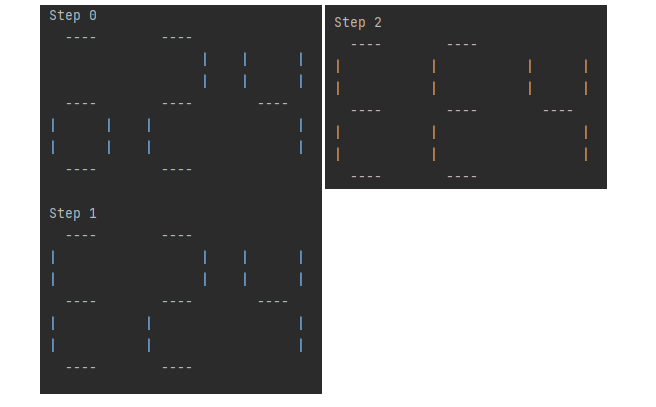
\includegraphics{result0}

\\\\
\subsection{hexmax1.txt}
Eingabe: 
$$
\mathrm{509C431B55}
$$
Ausgabe:
$$
\mathrm{FFFEA97B55}
$$
Anzahl Umlegungen: 8\\
Zeit (mit Ausgabe der Umlegungen): 16 ms
\\\\
Umlegungen: \\
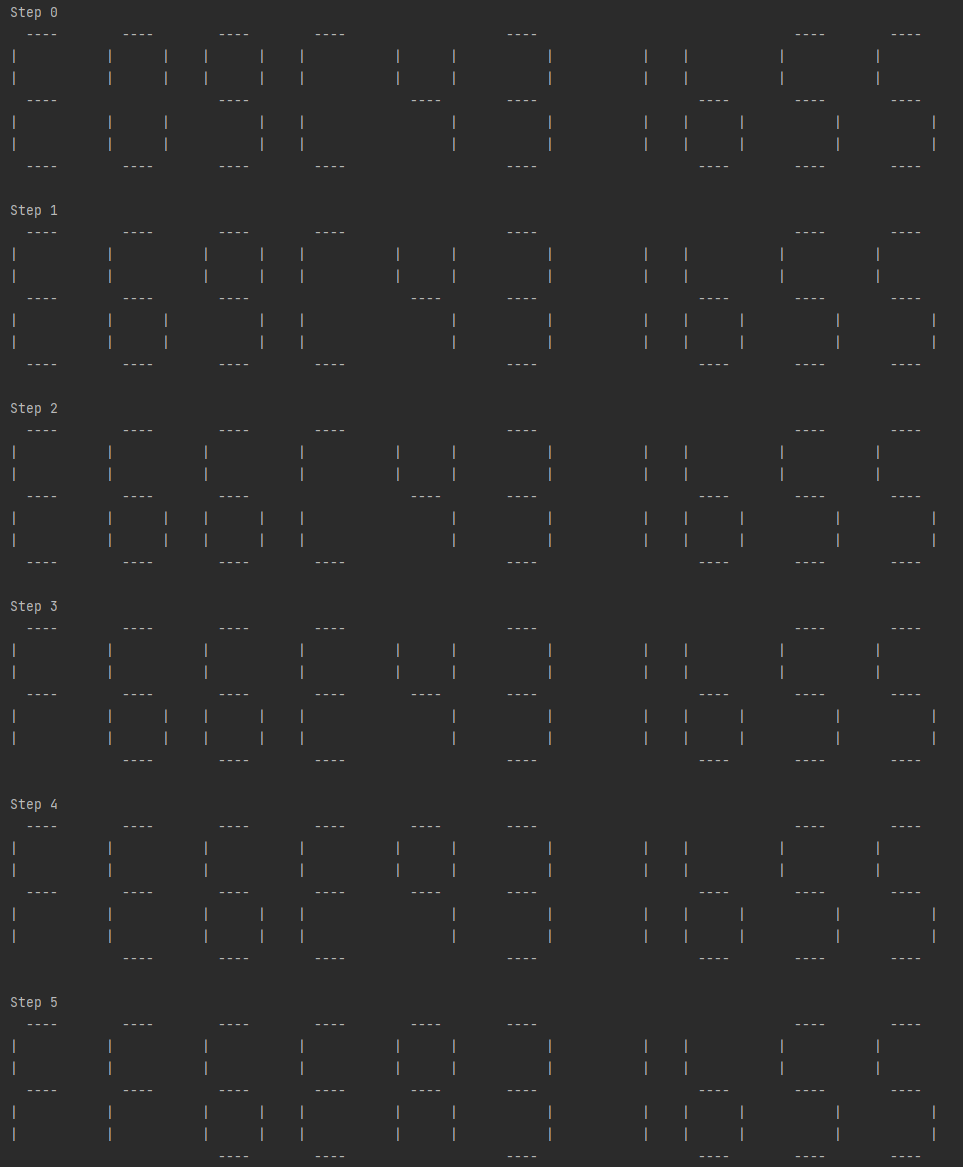
\includegraphics[width=15cm]{result1_1} \\
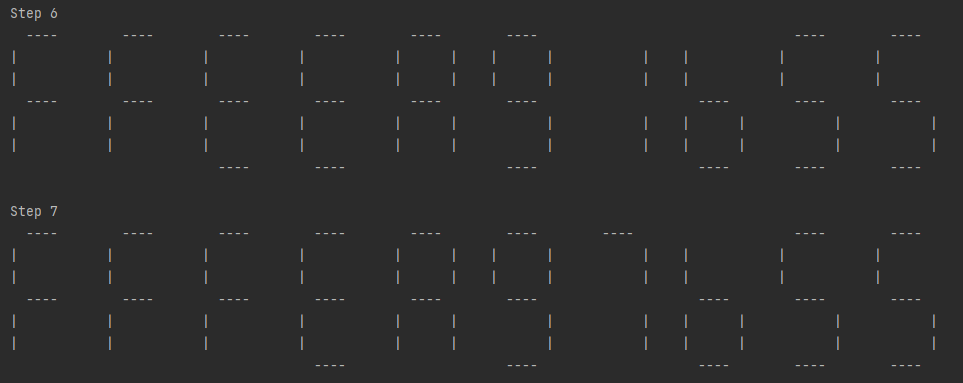
\includegraphics[width=15cm]{result1_2}

\\\\
\subsection{hexmax2.txt}
Eingabe: 
$$
\mathrm{632B29B38F11849015A3BCAEE2CDA0BD496919F8}
$$
Ausgabe:
$$
\mathrm{FFFFFFFFFFFFFFFFD9A9BEAEE8EDA8BDA989D9F8}
$$
Anzahl Umlegungen: 37
Zeit (mit Ausgabe der Umlegungen): 32 ms
\\\\
Umlegungen: \\
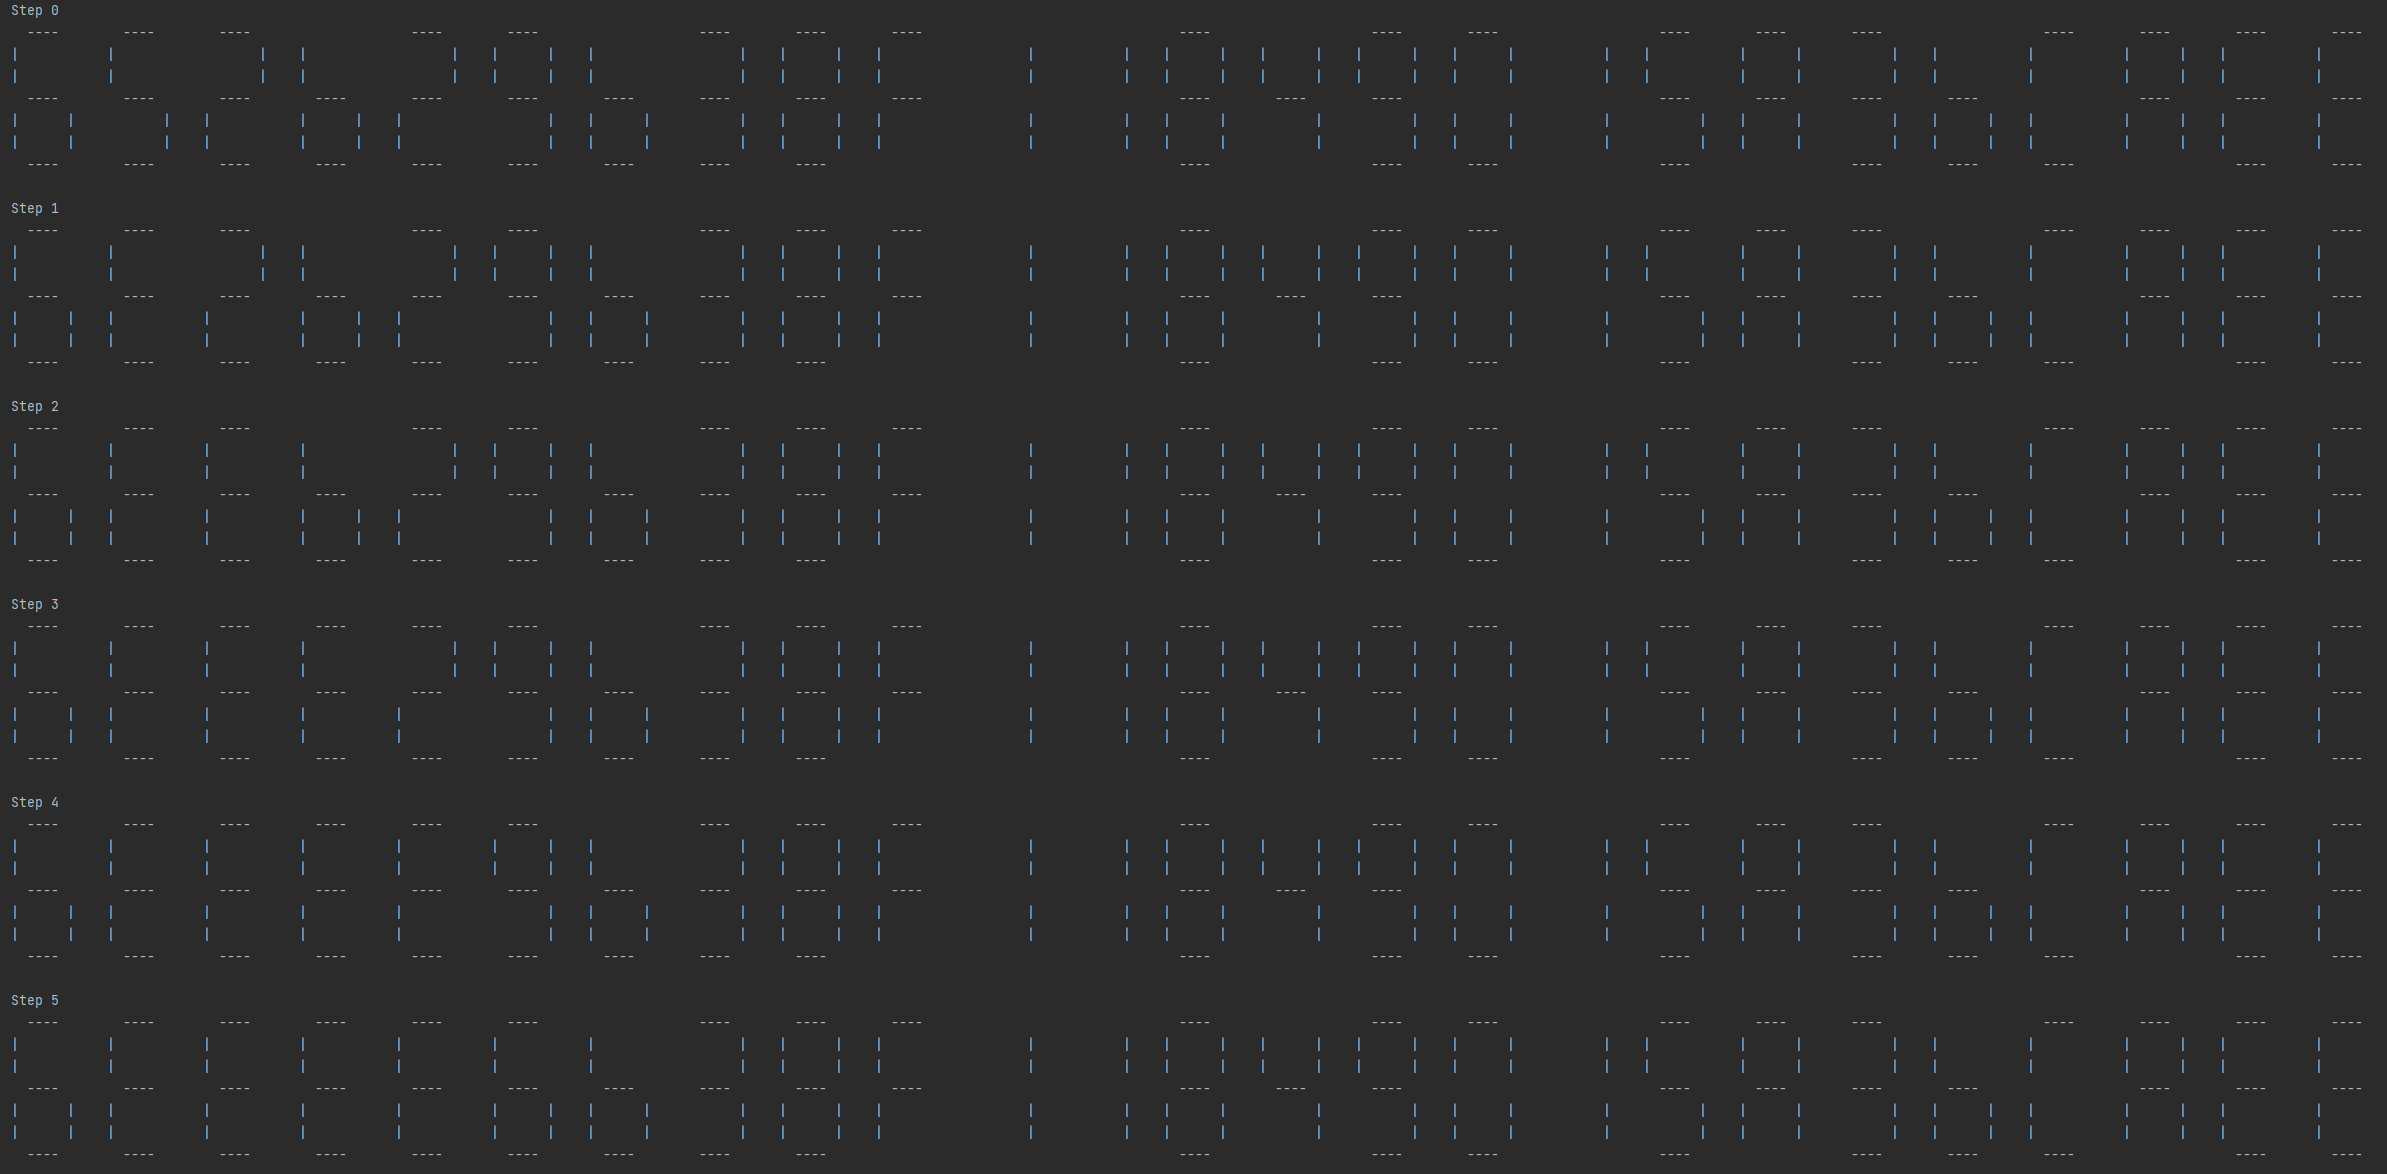
\includegraphics[width=9cm]{result2_1_1}
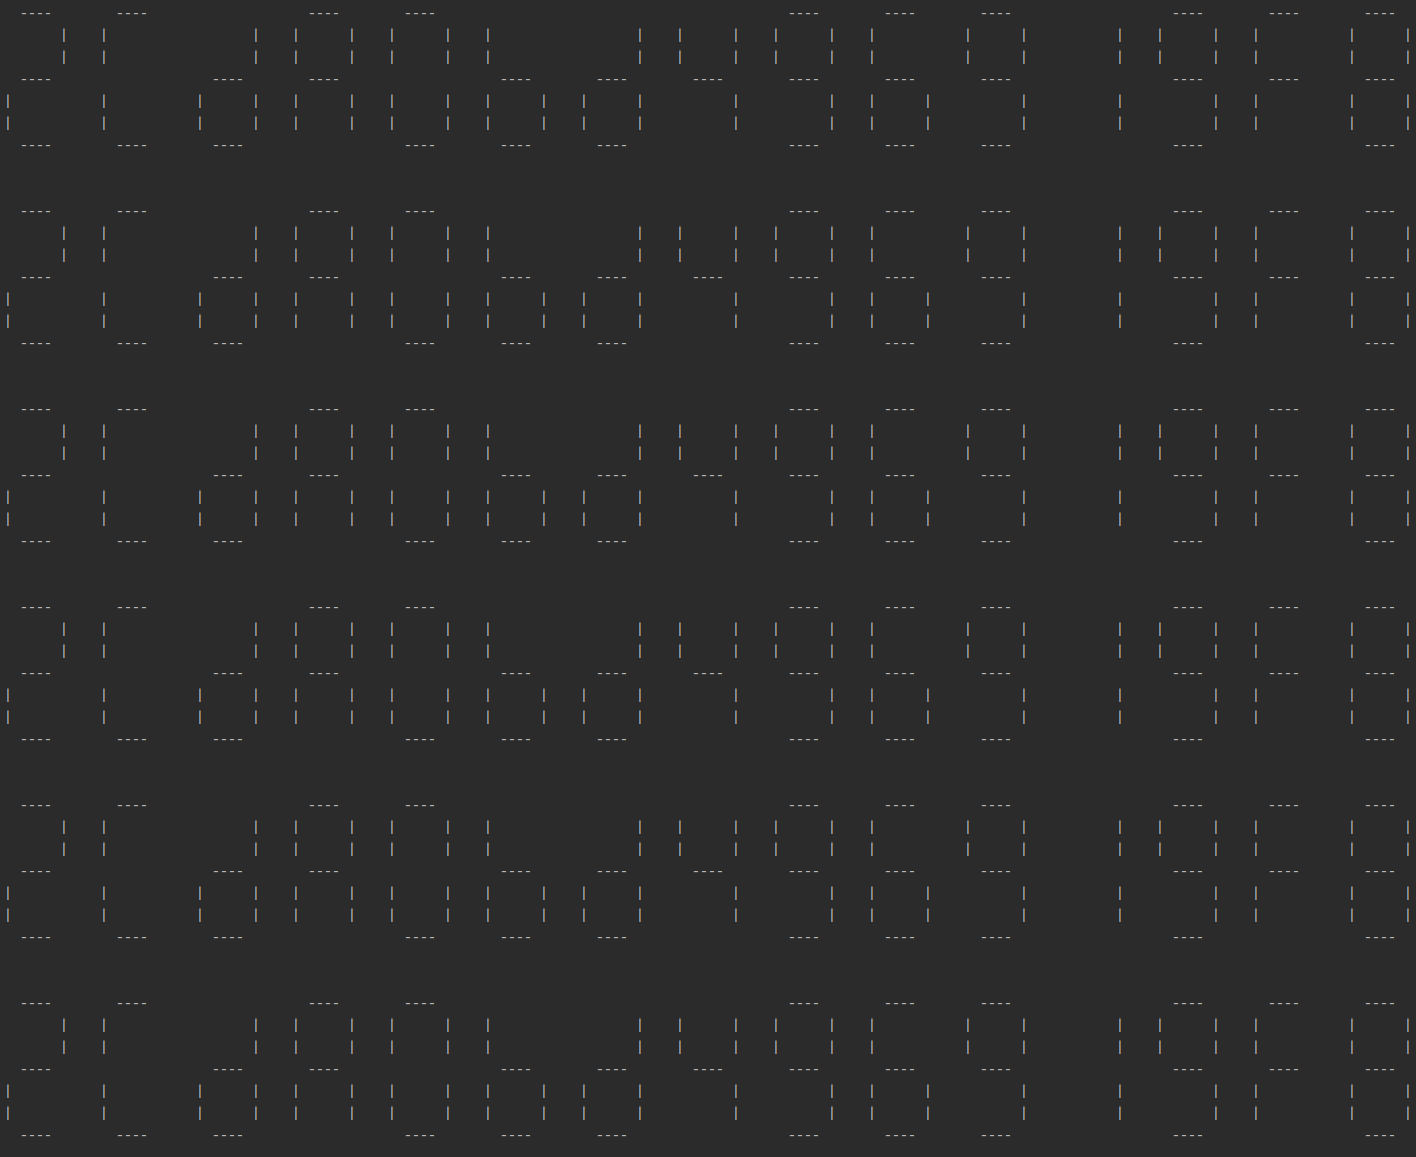
\includegraphics[width=5.4cm]{result2_1_2}
\\
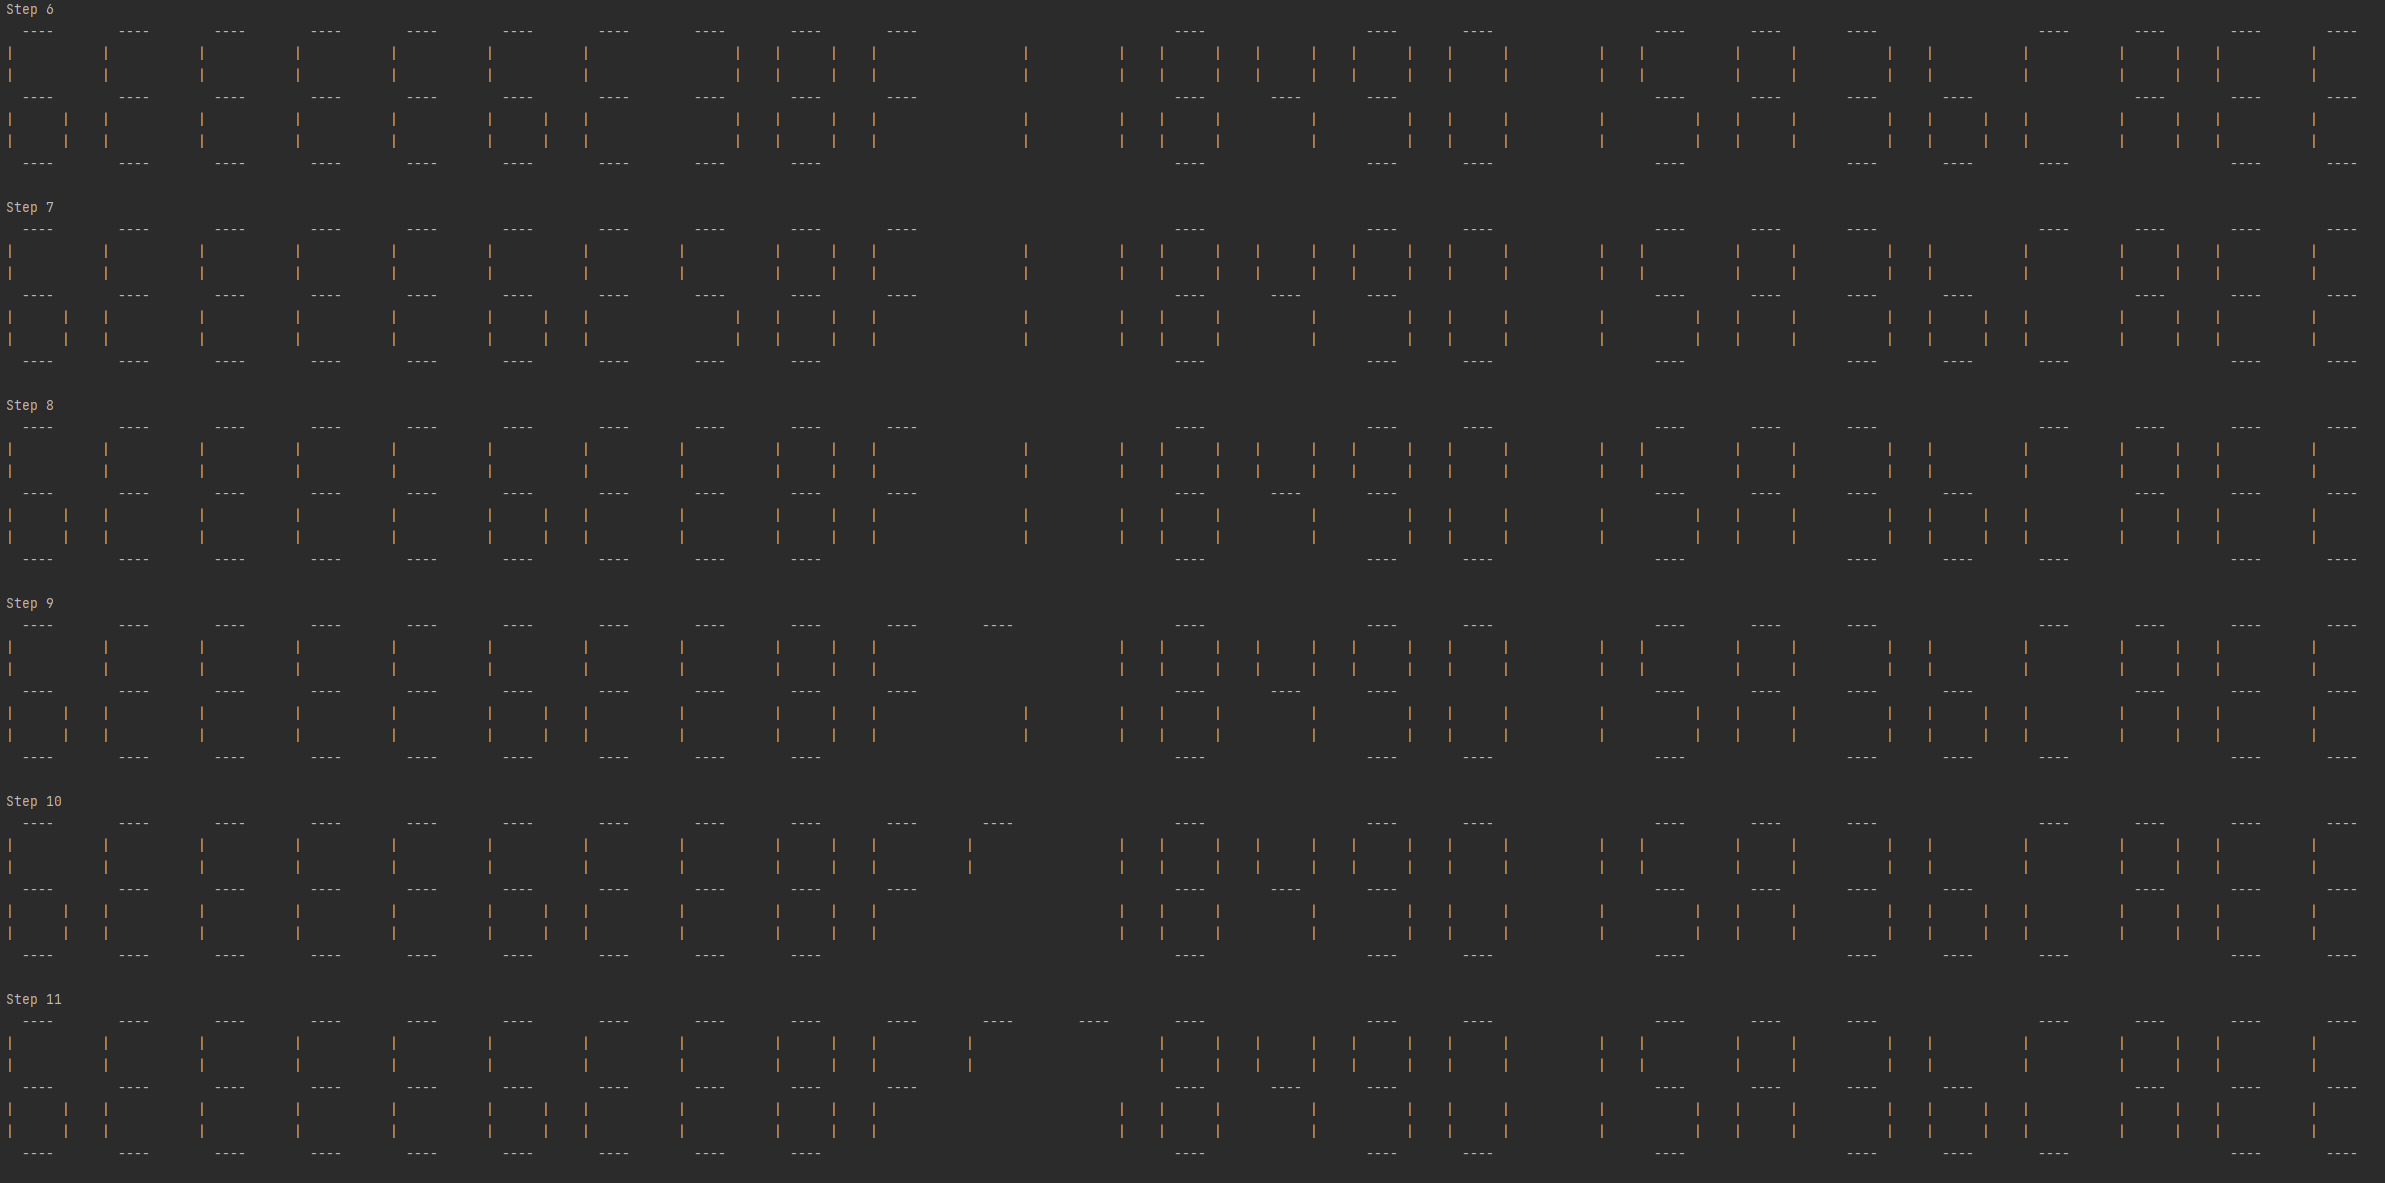
\includegraphics[width=9cm]{result2_2_1}
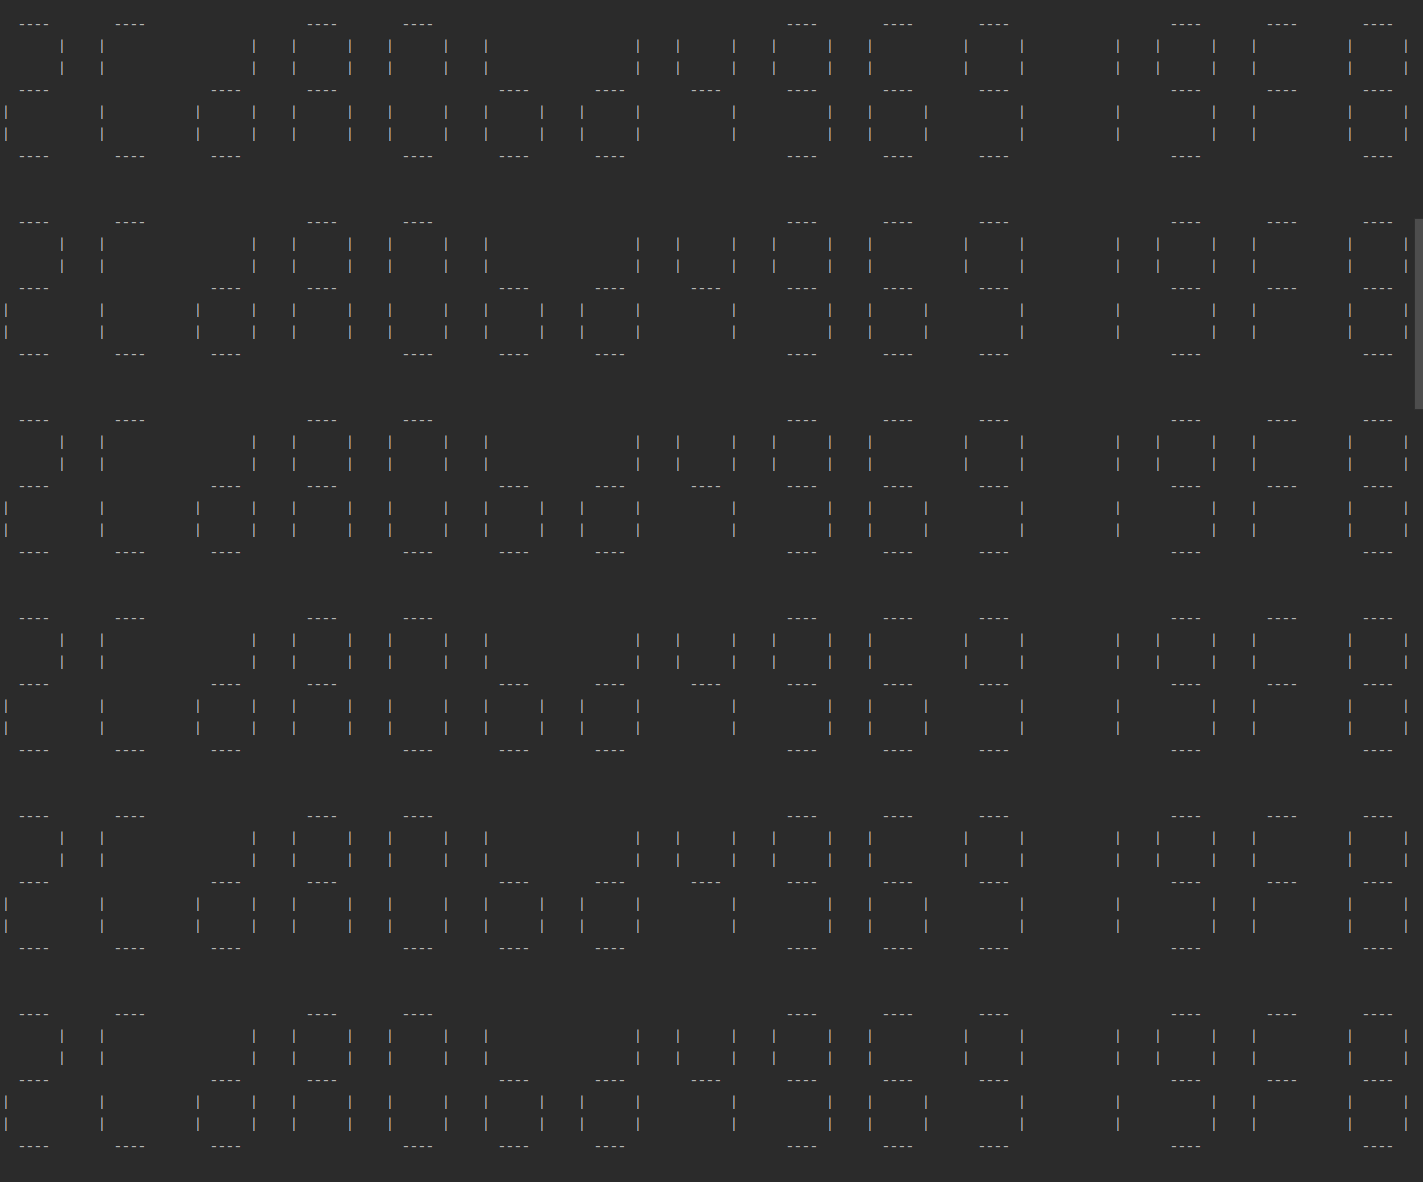
\includegraphics[width=5.4cm]{result2_2_2}
\\
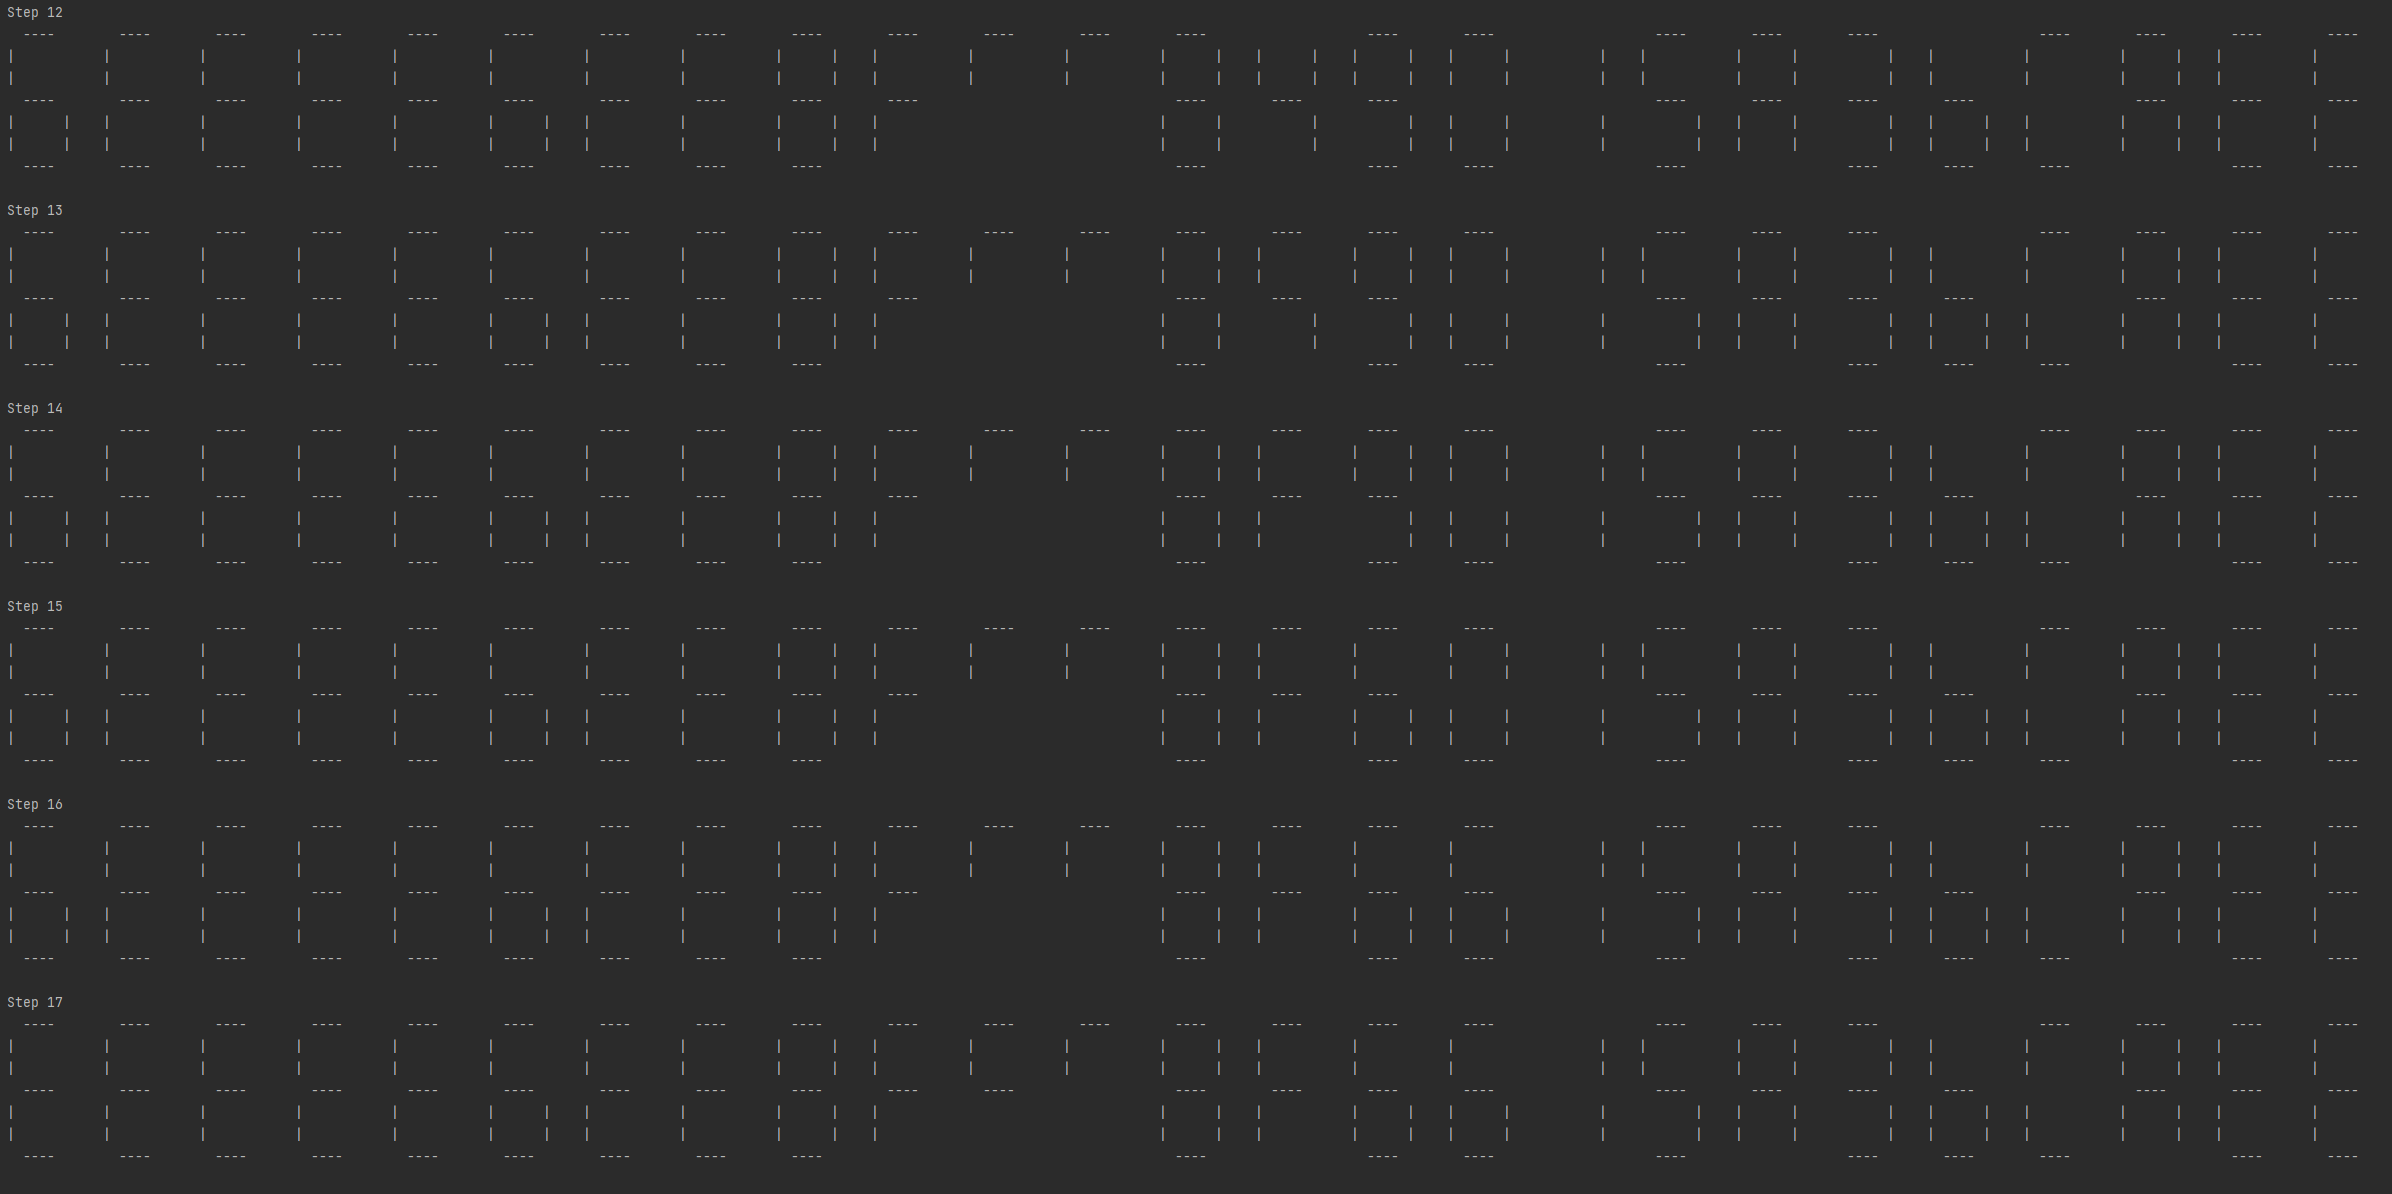
\includegraphics[width=9cm]{result2_3_1}
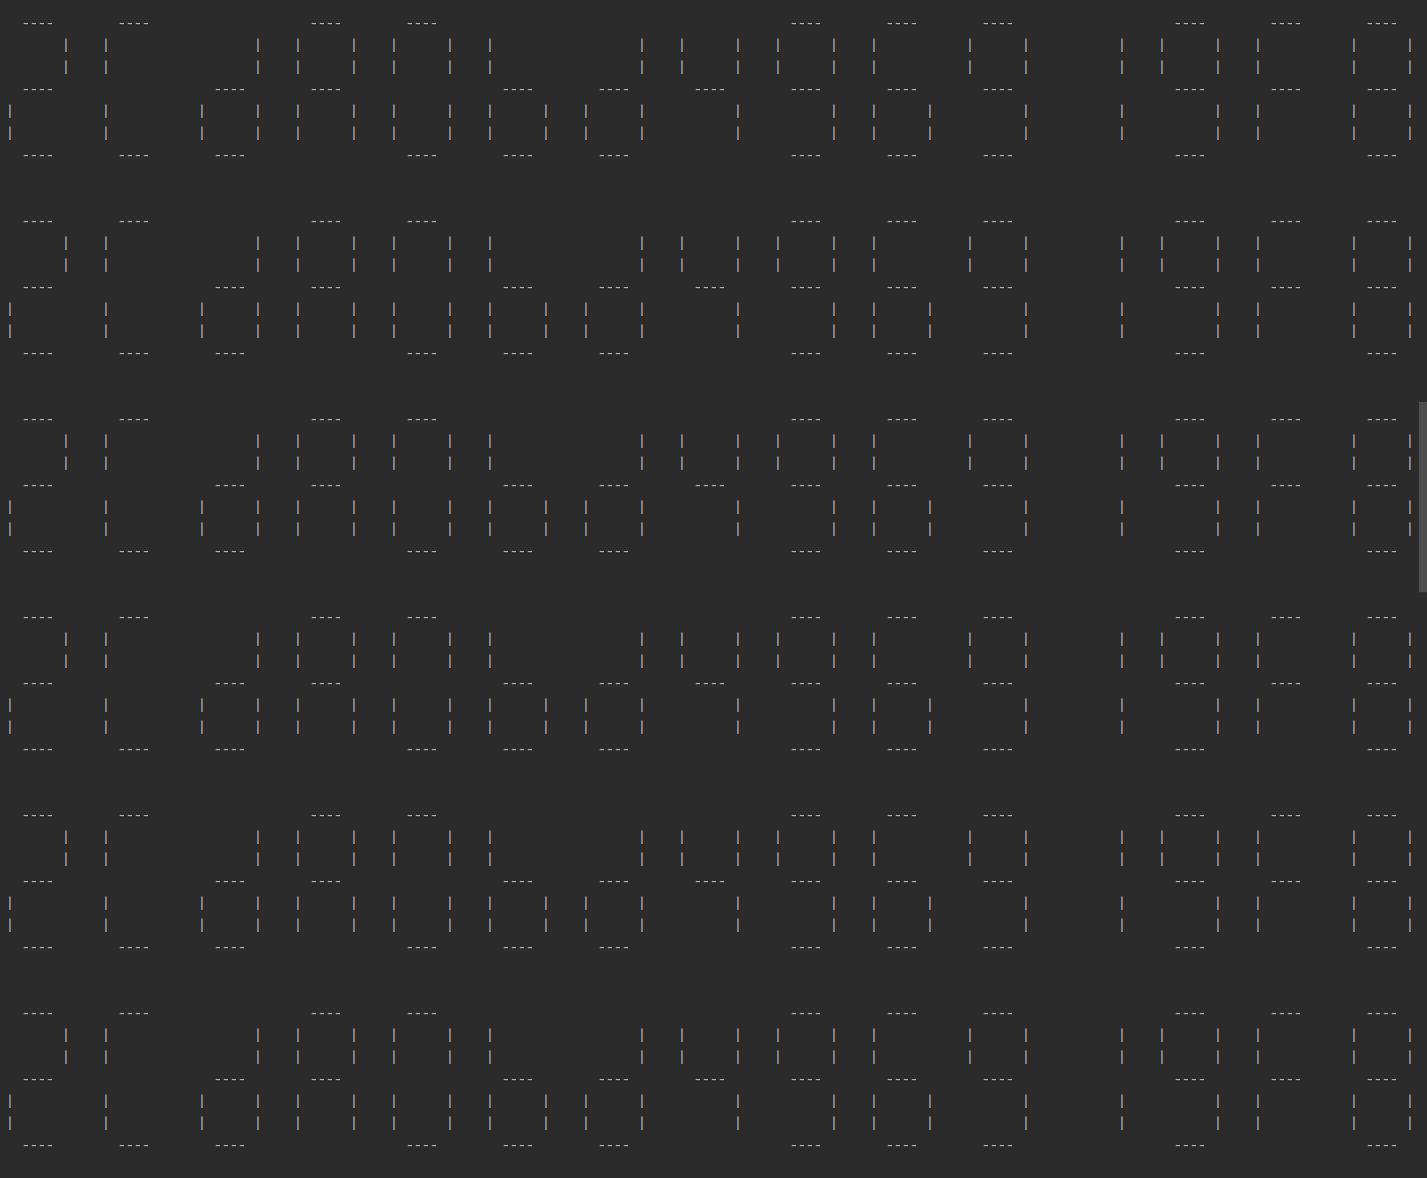
\includegraphics[width=5.4cm]{result2_3_2}
\\
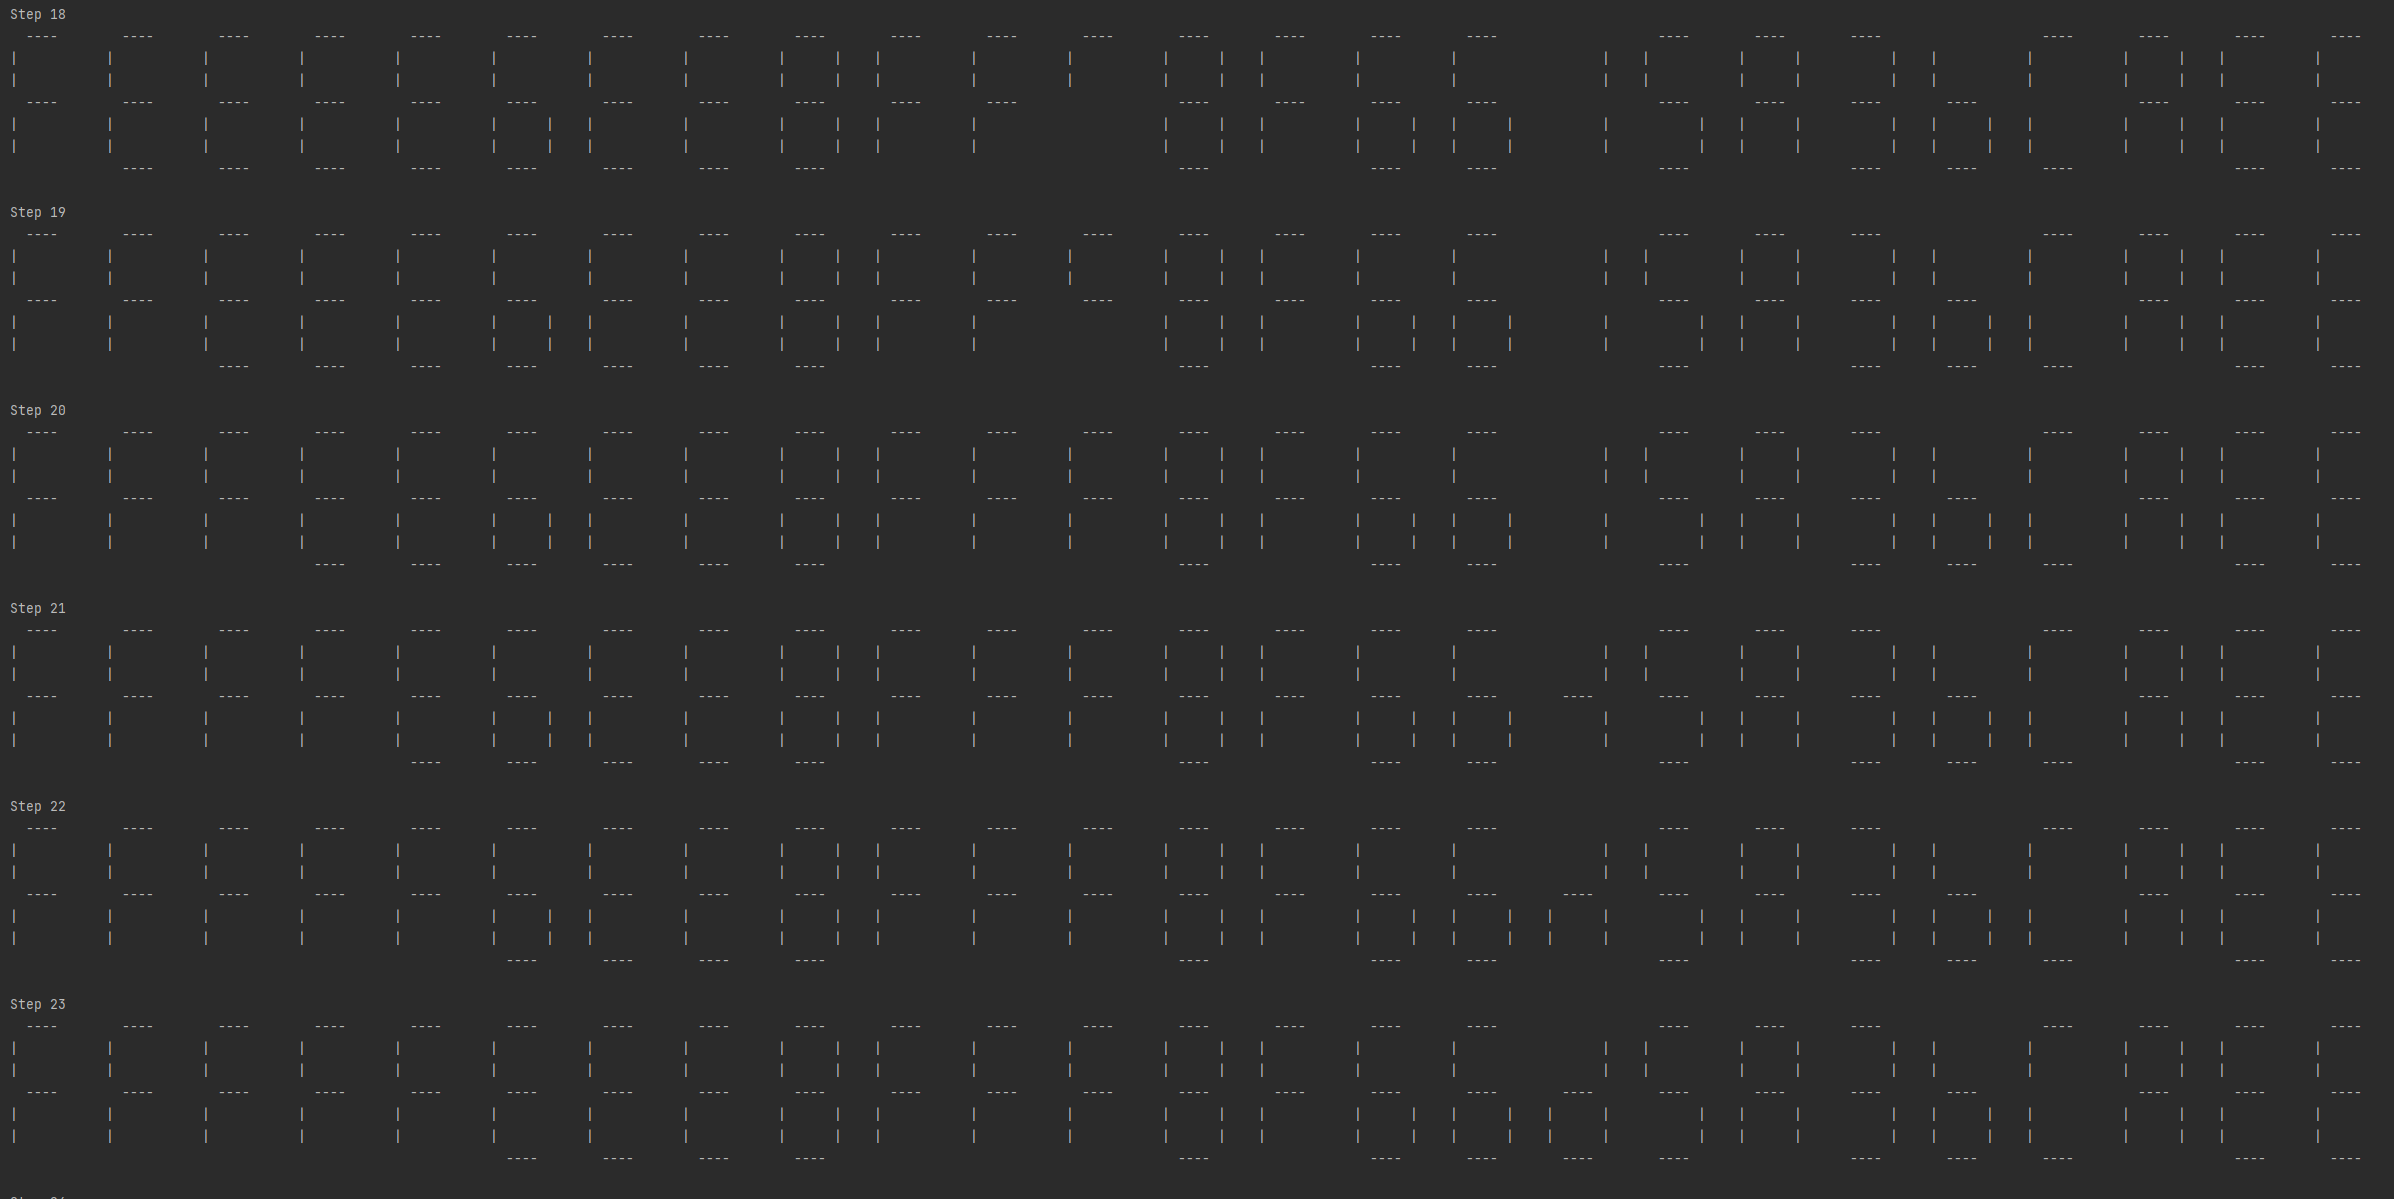
\includegraphics[width=9cm]{result2_4_1}
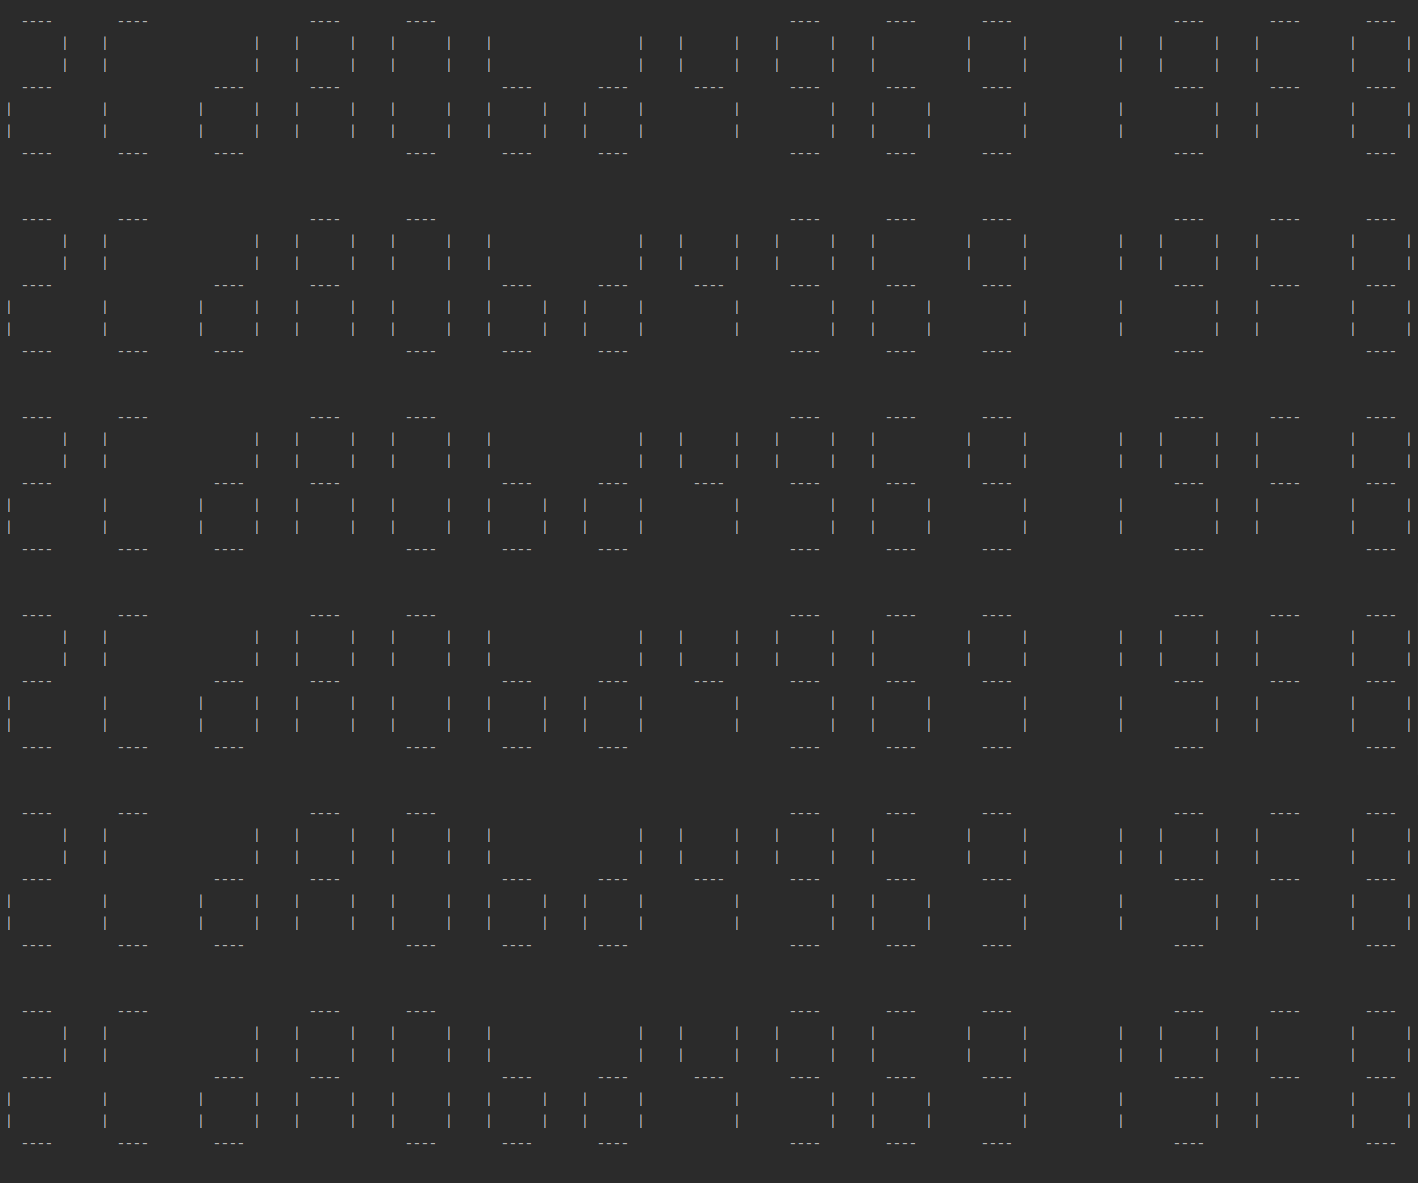
\includegraphics[width=5.4cm]{result2_4_2}
\\
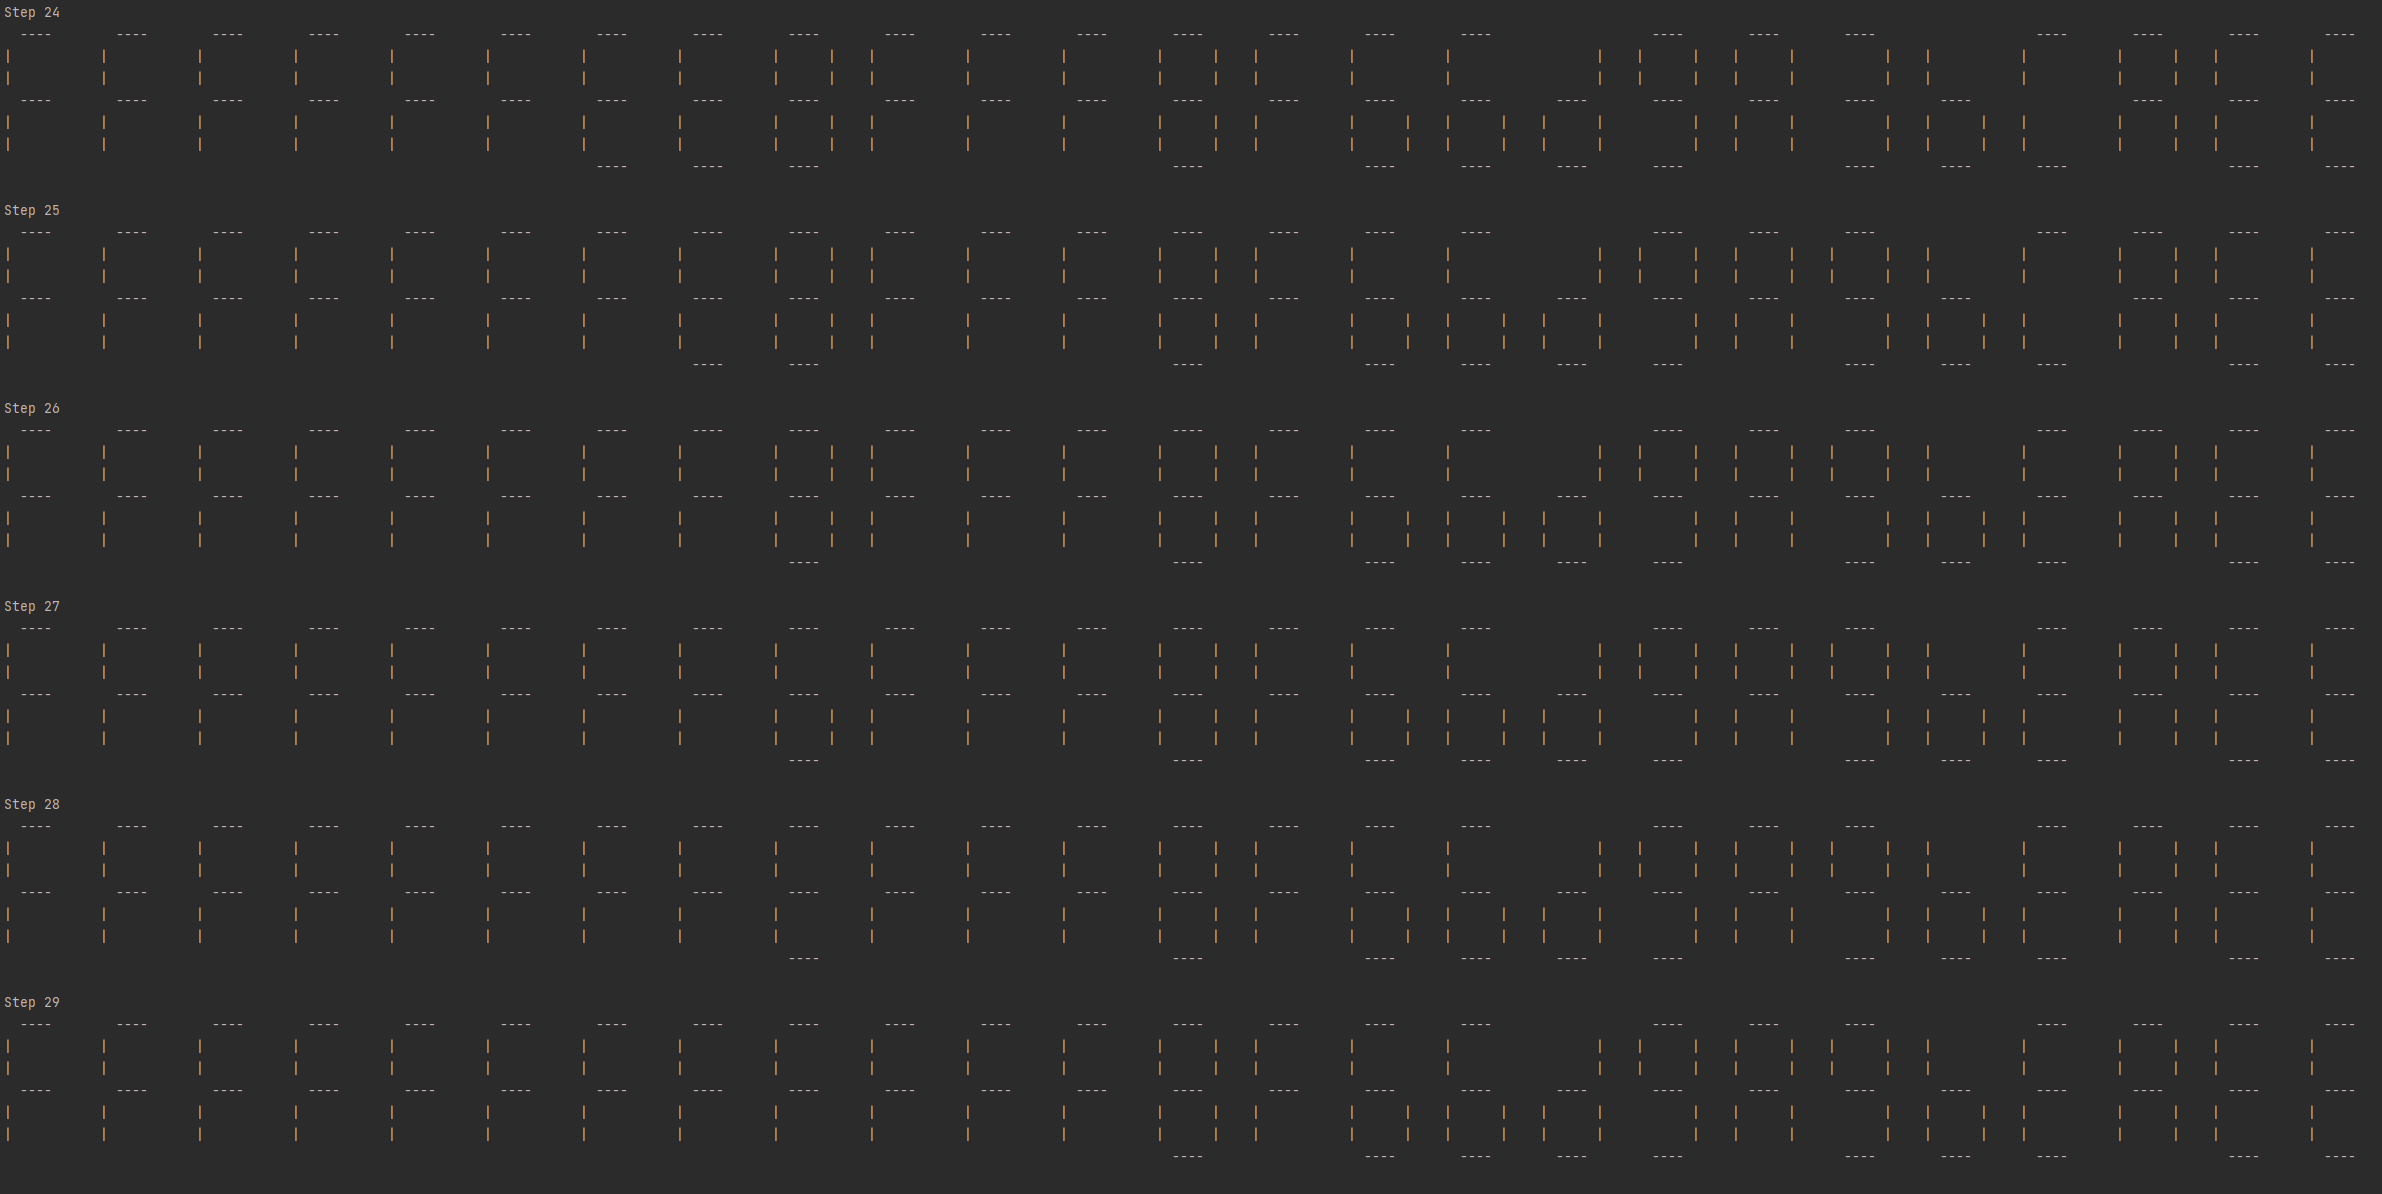
\includegraphics[width=9cm]{result2_5_1}
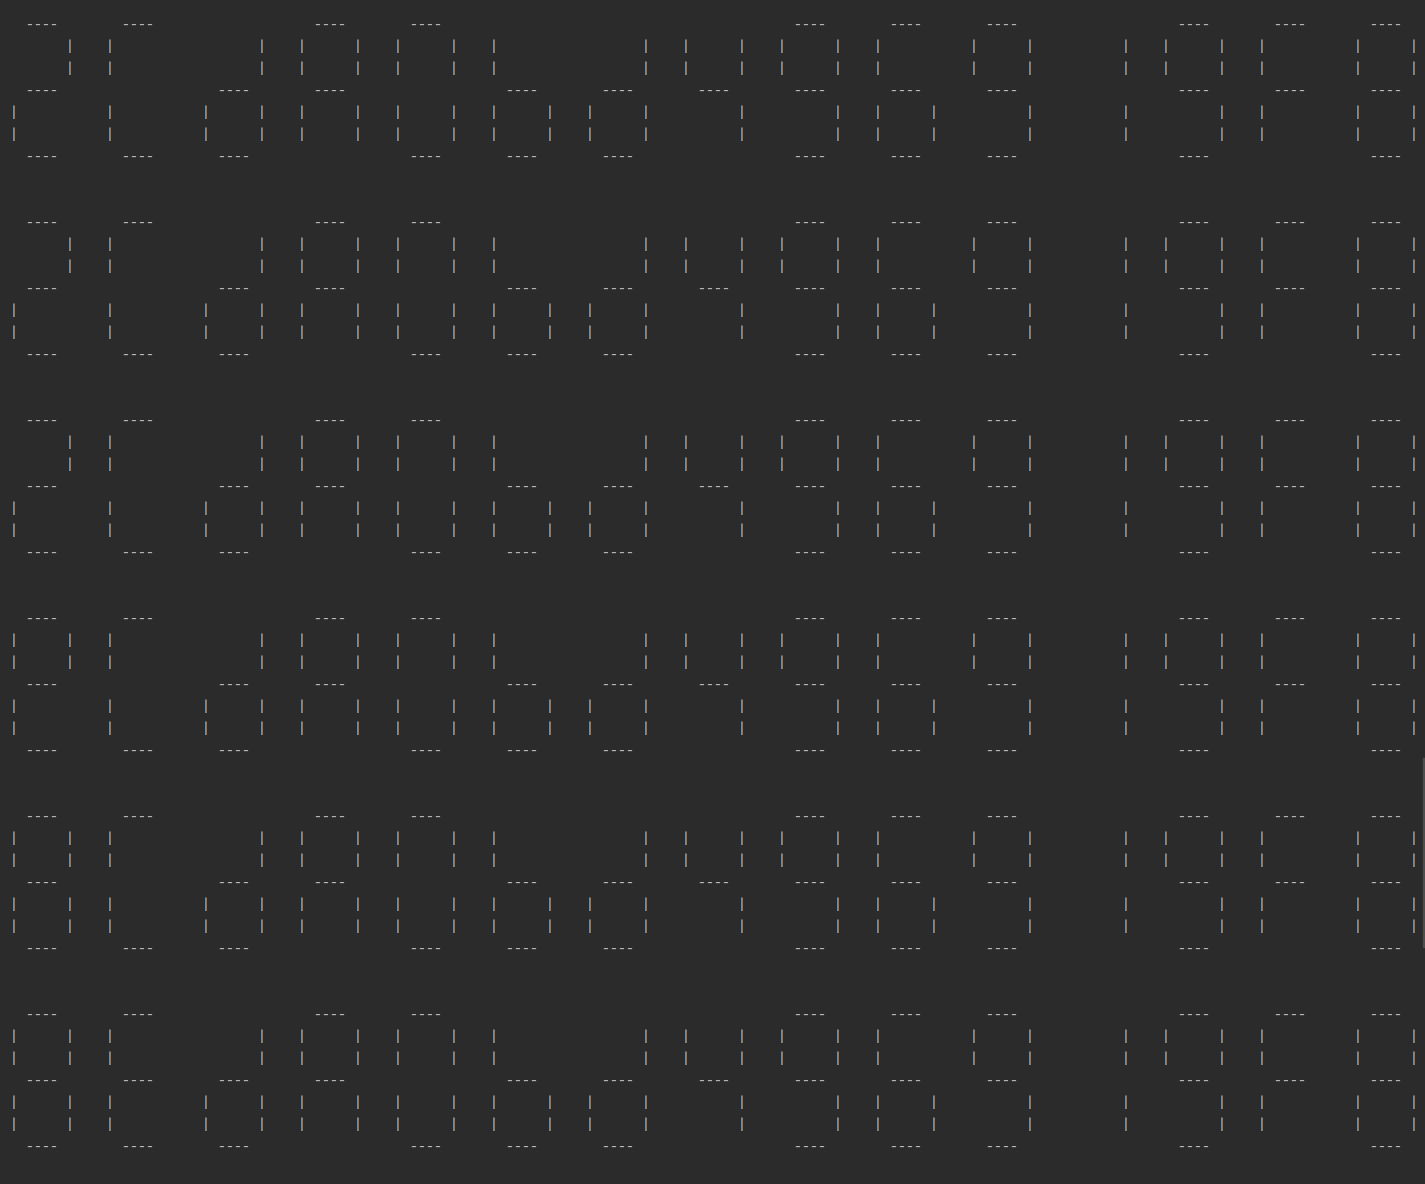
\includegraphics[width=5.4cm]{result2_5_2}
\\
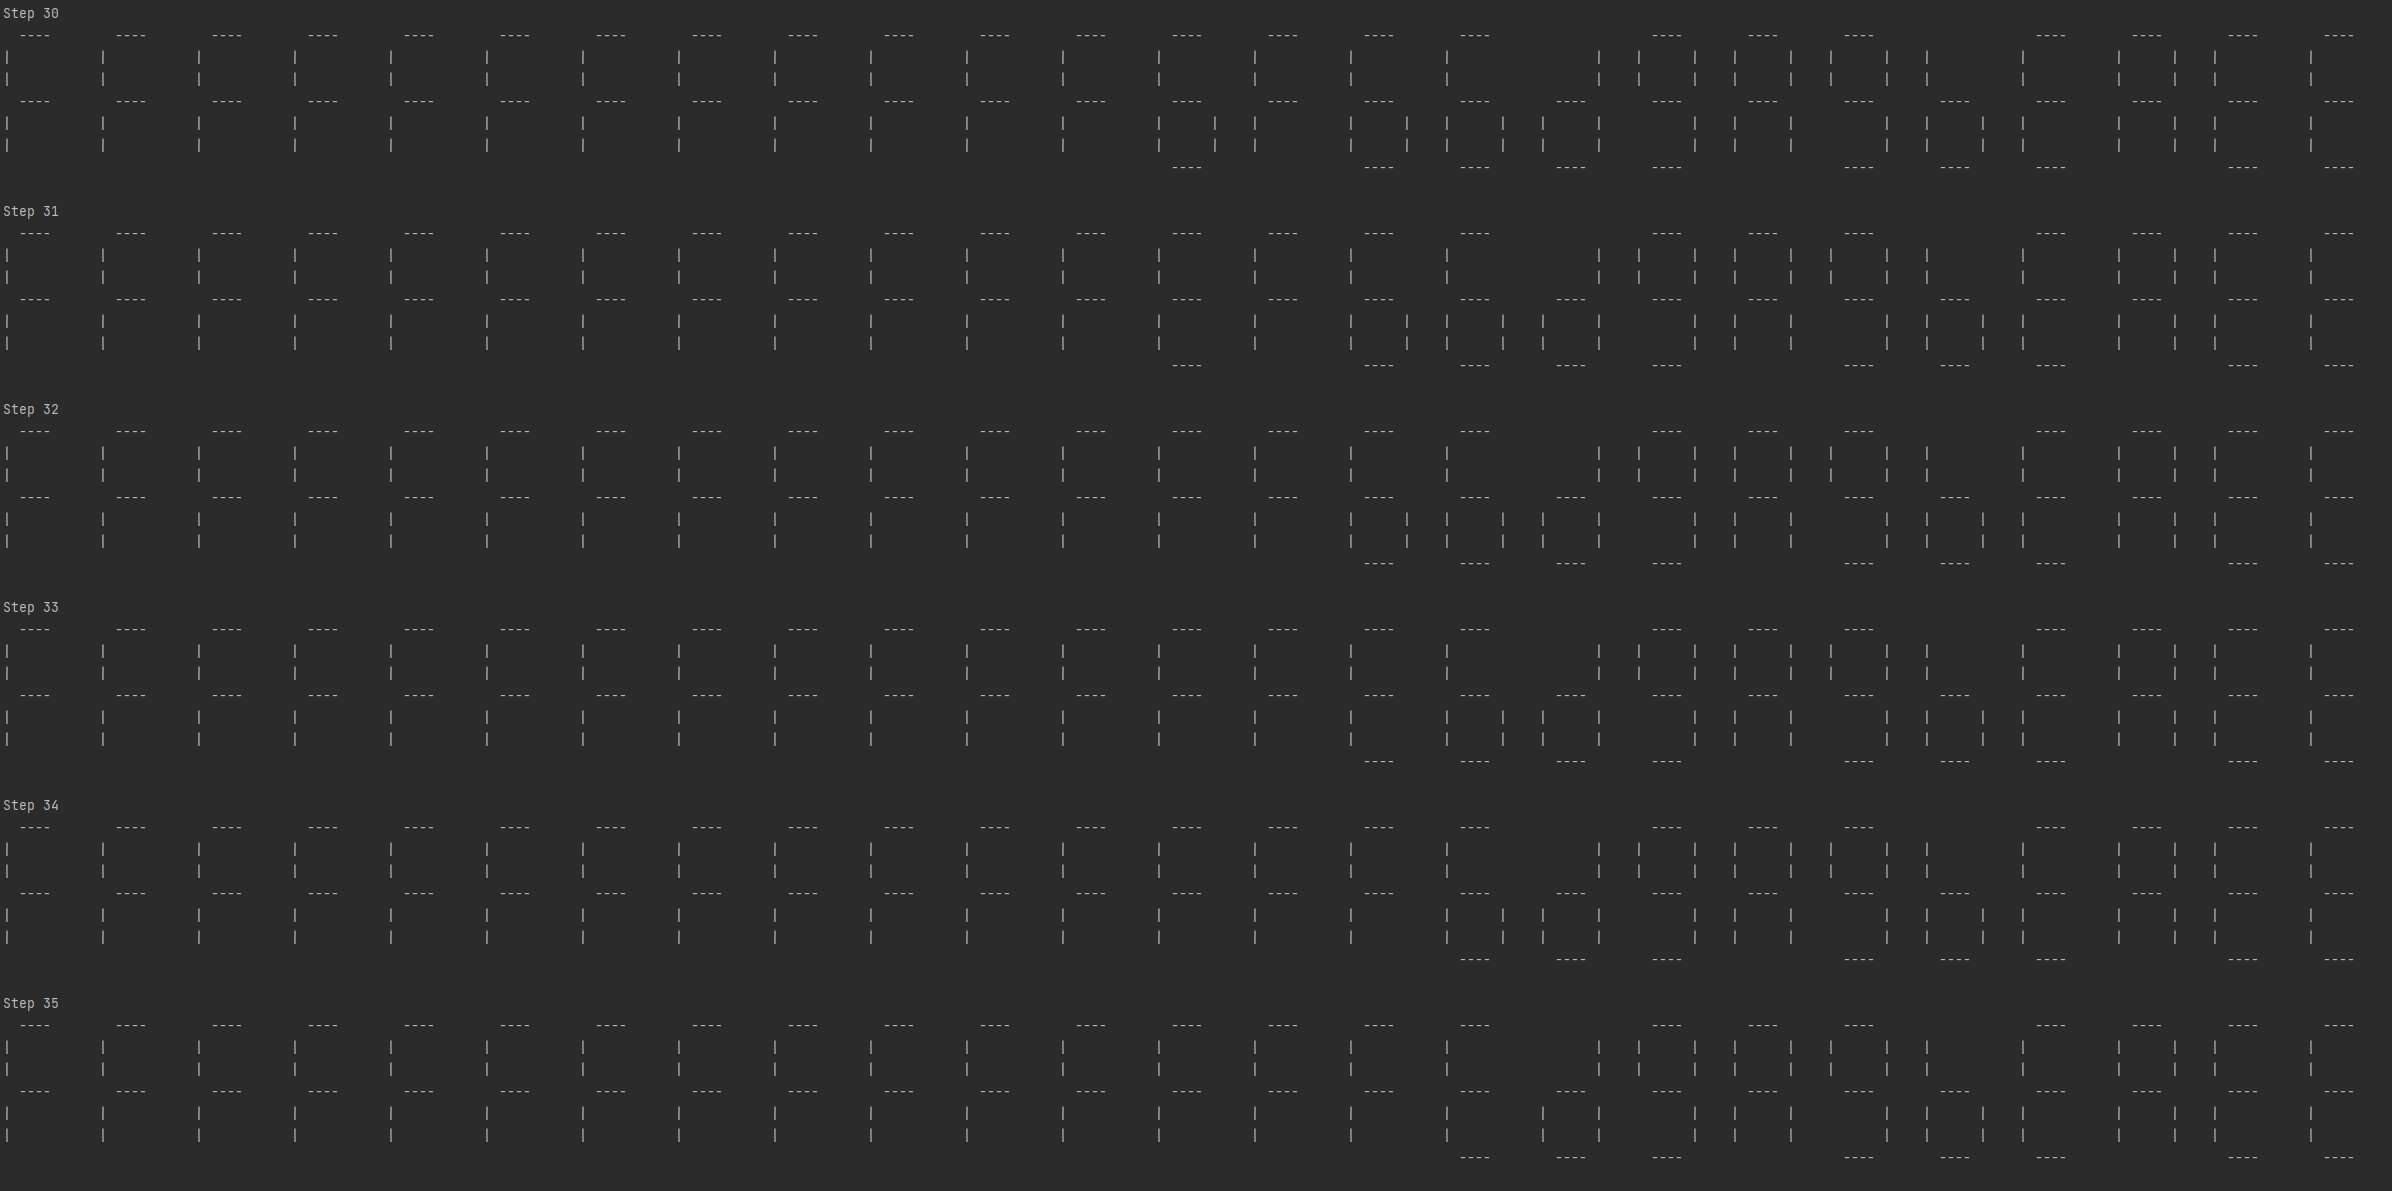
\includegraphics[width=9cm]{result2_6_1}
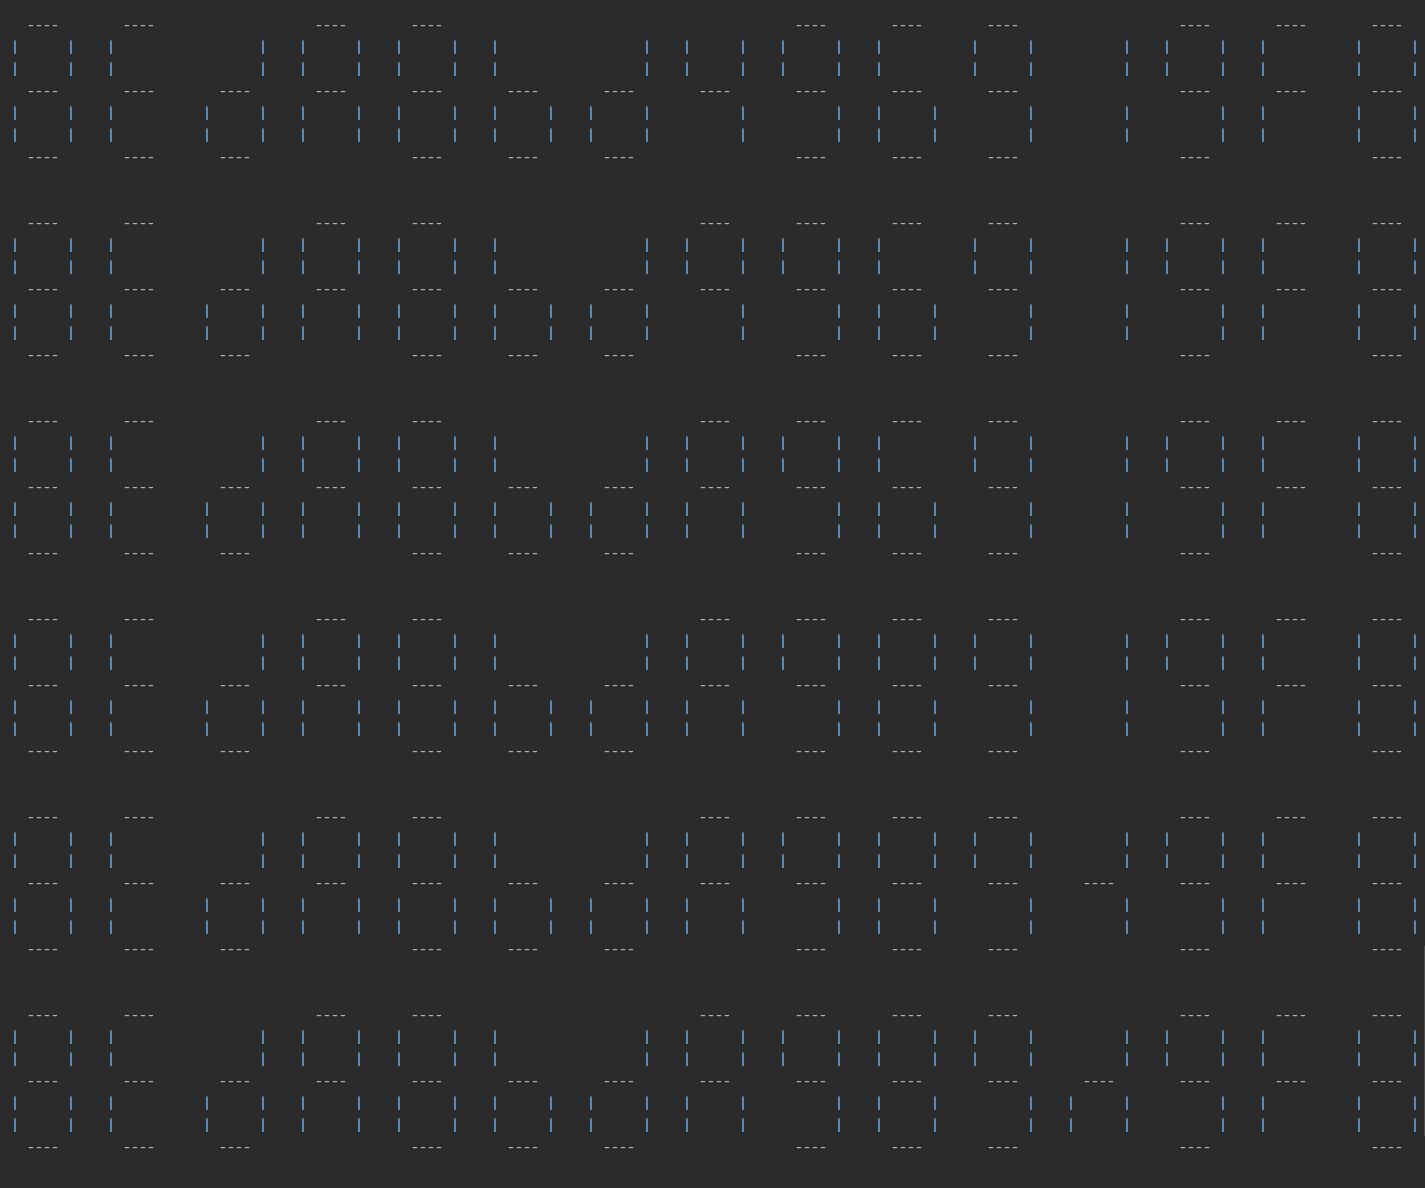
\includegraphics[width=5.4cm]{result2_6_2}
\\
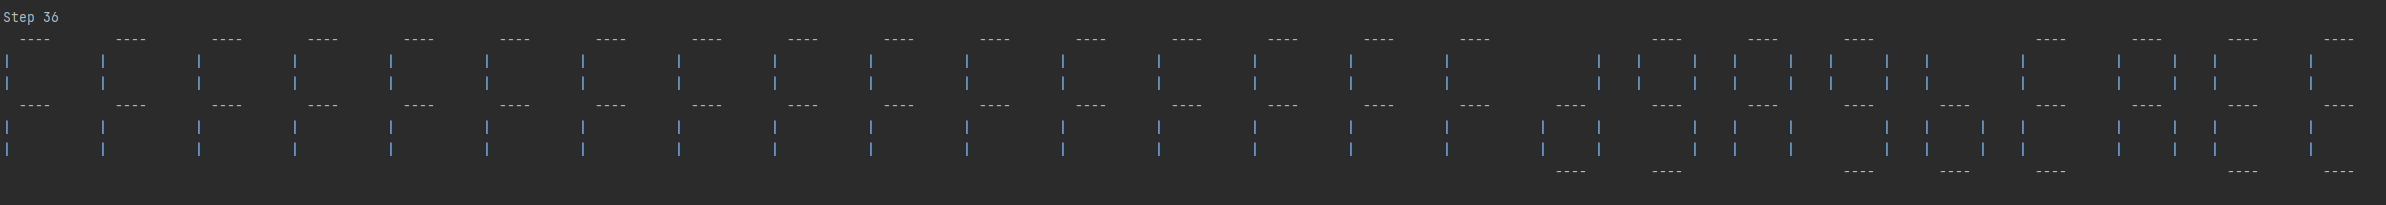
\includegraphics[width=9cm]{result2_7_1}
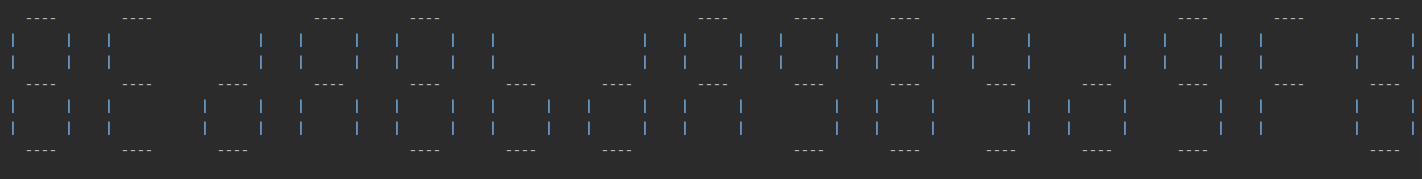
\includegraphics[width=5.4cm]{result2_7_2}

\\\\
\subsection{hexmax3.txt}
Eingabe:
$$
\mathrm{0E9F1DB46B1E2C081B059EAF198FD491F477CE1CD37EBFB65F}
$$
$$
\mathrm{8D765055757C6F4796BB8B3DF7FCAC606DD0627D6B48C17C09}
$$
Ausgabe:
$$
\mathrm{FFFFFFFFFFFFFFFFFFFFFFFFFFFFFFFFFFFFFFFFFFFFFFFFFF}
$$
$$
\mathrm{FFFFFFFFFFFFFFAA98BB8B9DFAFEAE888DD888AD8BA8EA8888}
$$
Anzahl Umlegungen: 121\\
Zeit (ohne Ausgabe der Umlegungen): 48 ms
\\\\

\subsection{hexmax4.txt}
Eingabe:
$$
\mathrm{1A02B6B50D7489D7708A678593036FA265F2925B21C28B4724}
$$
$$
\mathrm{DD822038E3B4804192322F230AB7AF7BDA0A61BA7D4AD8F888}
$$
Ausgabe:
$$
\mathrm{FFFFFFFFFFFFFFFFFFFFFFFFFFFFFFFFFFFFFFEB8DE88BAA8A}
$$
$$
\mathrm{DD888898E9BA88AD98988F898AB7AF7BDA8A61BA7D4AD8F888}
$$
Anzahl Umlegungen: 87\\
Zeit (ohne Ausgabe der Umlegungen): 77 ms
\\\\

\subsection{hexmax5.txt}
Eingabe:
$$
\mathrm{EF50AA77ECAD25F5E11A307B713EAAEC55215E7E640FD263FA}
$$
$$
\mathrm{529BBB48DC8FAFE14D5B02EBF792B5CCBBE9FA1330B867E330}
$$
$$
\mathrm{A6412870DD2BA6ED0DBCAE553115C9A31FF350C5DF99382488}
$$
$$
\mathrm{6DB5111A83E773F23AD7FA81A845C11E22C4C45005D192ADE6}
$$
$$
\mathrm{8AA9AA57406EB0E7C9CA13AD03888F6ABEDF1475FE9832C66B}
$$
$$
\mathrm{FDC28964B7022BDD969E5533EA4F2E4EABA75B5DC119728248}
$$
$$
\mathrm{96786BD1E4A7A7748FDF1452A5079E0F9E6005F040594185EA}
$$
$$
\mathrm{03B5A869B109A283797AB31394941BFE4D38392AD12186FF6D}
$$
$$
\mathrm{233585D8C820F197FBA9F6F063A0877A912CCBDCB14BEECBAE}
$$
$$
\mathrm{C0ED061CFF60BD517B6879B72B9EFE977A9D3259632C718FBF}
$$
$$
\mathrm{45156A16576AA7F9A4FAD40AD8BC87EC569F9C1364A63B1623}
$$
$$
\mathrm{A5AD559AAF6252052782BF9A46104E443A3932D25AAE8F8C59}
$$
$$
\mathrm{F10875FAD3CBD885CE68665F2C826B1E1735EE2FDF0A196514}
$$
$$
\mathrm{9DF353EE0BE81F3EC133922EF43EBC09EF755FBD740C8E4D02}
$$
$$
\mathrm{4B033F0E8F3449C94102902E143433262CDA1925A2B7FD01BE}
$$
$$
\mathrm{F26CD51A1FC22EDD49623EE9DEB14C138A7A6C47B677F033BD}
$$
$$
\mathrm{EB849738C3AE5935A2F54B99237912F2958FDFB82217C17544}
$$
$$
\mathrm{8AA8230FDCB3B3869824A826635B538D47D847D8479A88F350}
$$
$$
\mathrm{E24B31787DFD60DE5E260B265829E036BE340FFC0D8C05555E}
$$
$$
\mathrm{75092226E7D54DEB42E1BB2CA9661A882FB718E7AA53F1E606}
$$
Ausgabe:
$$
\mathrm{FFFFFFFFFFFFFFFFFFFFFFFFFFFFFFFFFFFFFFFFFFFFFFFFFF}
$$
$$
\mathrm{FFFFFFFFFFFFFFFFFFFFFFFFFFFFFFFFFFFFFFFFFFFFFFFFFF}
$$
$$
\mathrm{FFFFFFFFFFFFFFFFFFFFFFFFFFFFFFFFFFFFFFFFFFFFFFFFFF}
$$
$$
\mathrm{FFFFFFFFFFFFFFFFFFFFFFFFFFFFFFFFFFFFFFFFFFFFFFFFFF}
$$
$$
\mathrm{FFFFFFFFFFFFFFFFFFFFFFFFFFFFFFFFFFFFFFFFFFFFFFFFFF}
$$
$$
\mathrm{FFFFFFFFFFFFFFFFFFFFFFFFFFFFFFFFFFFFFFFFFFFFFFFFFF}
$$
$$
\mathrm{FFFFFFFFFFFFFFFFFFFFFFFFFFFFFFFFFFFFFFFFFFFFFFFFFF}
$$
$$
\mathrm{FFFFFFFFFFFFFFFFFFFFFFFFFFFFFFFFFFFFFFFFFFFFFFFFFF}
$$
$$
\mathrm{FFFFFFFFFFFFFFFFFFFFFFFFFFFFFFFFFFFFFFFFFFFFFFFFFF}
$$
$$
\mathrm{FFFFFFFFFFFFFFFFFFFFFFFFFFFFFFFFFFFFFFFFFFFFFFFFFF}
$$
$$
\mathrm{FFFFFFFFFFFFFFFFFFFFFFFFFFFFFFFFFFFFFFFFFFFFFFFFFF}
$$
$$
\mathrm{FFFFFFFFFFFFFFFFFFFFFFFFFFFFFFFFFFFFFFFFFFFFFFFFFF}
$$
$$
\mathrm{FFFFFFFFFFFFFFFFFFFFFFFFFFFFFFFFFFFFFFFFFFFFFFFFFF}
$$
$$
\mathrm{FFFFFFFFFFFFFFFFFFFFF88EFA9EBE89EFA99FBDAA8E8EAD88}
$$
$$
\mathrm{AB899F8E8F9AA9E9AD88988EDA9A99888EDAD989A8BAFD8A88}
$$
$$
\mathrm{88888888888888888888888888888888888888888888888888}
$$
$$
\mathrm{88888888888888888888888888888888888888888888888888}
$$
$$
\mathrm{88888888888888888888888888888888888888888888888888}
$$
$$
\mathrm{88888888888888888888888888888888888888888888888888}
$$
$$
\mathrm{88888888888888888888888888888888888888888888888888}
$$
Anzahl Umlegungen: TEST2 - 1369 \\
Zeit (ohne Ausgabe der Umlegungen):  62,6 s
\\\\



\end{document}
